%%%%%%%%%%%%%%%%%%%%%%%%%%%%%%%%%%%%%%%%%%%%%%%%%%%%%%%%%%%%%%%%%%%%%%%%%%%%%%%%
% LPL-Vorlage: Wissenschaftliche Arbeit. angepasst auf Basis der TUM-Vorlage
%%%%%%%%%%%%%%%%%%%%%%%%%%%%%%%%%%%%%%%%%%%%%%%%%%%%%%%%%%%%%%%%%%%%%%%%%%%%%%%%




% BASIC SETUP
% DO NOT ALTER UNLESS YOU KNOW WHAT YOU DO!
% (In that case, feel free to fiddle around and adapt to your needs)
%%%%%%%%%%%%%%%%%%%%%%%%%%%%%%%%%%%%%%%%%%%%%%%%%%%%%%%%%%%%%%%%%%%%%%%%%%%%%%%%
\documentclass[%
	a4paper, % Papierformat
	12pt, % Standard-Schriftgröße
	DIV=14, % Seitenspiegel angepasst (bei DIV=calc wird DIV nach der Schriftdefinition berechnet mit \typearea[current]{calc}
	twoside, % gespiegelte Seitenränder
%	open=right, % Kapitel immer auf der rechten Seite beginnen
	BCOR=8mm, % Bindekorrektur
	headsepline, % Linie unterhalb von Kopfzeile
	footsepline, % Linie überhalb der Fußzeile
%	headinclude, % Kofpzeile und...
%	footinclude, % Fußzeile bei Berechnung von Satzspiegel berücksichtigt (führt zu größerem Rand)
	parskip=full, % Absätze sind deutlicher
%	numbers=noendperiod, % kein automatischer Punkt nach Gliederungsnummer
	headings=small,
	toc=chapterentrydotfill, % Punkte bis zur Seitennummer bei Kapiteln
	toc=listofnumbered,
	toc = bibliographynumbered,
	listof=entryprefix, % Präfix für Einträge in Abbildungs- und Tabellenverzeichnis
	listof=nochaptergap % Abstand für Kapiteleinträge in extra Verzeichnissen
	numbers=noendperiod, % kein automatischer Punkt nach Gliederungsnummer
%	appendixprefix = true
]{scrreprt} % Dokumentenart



%%%% PACKAGES %%%%%
\usepackage[T1]{fontenc} % Europäische Zeichensätze und Silbentrennung
\usepackage[utf8]{inputenc} % deutsche Sonderzeichen
\usepackage[ngerman, english]{babel} % dito

% Schriftart
%\usepackage{lmodern} % Schriftart Latin Modern
\usepackage{mathptmx} % Schriftart Helvetica
\usepackage[scaled=0.9]{helvet}
%\usepackage[scaled=0.78]{luximono} % Typewriter-Schriftart
\usepackage{courier} % Typewriter-Schriftart

%\typearea[current]{calc} % berechne nun Satzspiegel aufgrund der gewählten Schriftart, falls DIV=calc gewählt in \documentclass[options]

\usepackage{amsmath}  % MACHT
\usepackage{amsfonts} %		MATHE
\usepackage{amssymb}  %			MÄCHTIGER
\usepackage{stmaryrd} % ...und noch eine Menge nützlicher Symbole
\usepackage{mathtools}

\usepackage{blindtext} % Kann Blindtext einfügen (macht Formatierungen besser sichtbar)
\usepackage[table]{xcolor} % mehr Optionen für Tabellenumgebungen (zB für Tabellen, aber auch für Pakete wie listings oder pgfplotstable)

\usepackage{listings} % Code-Umgebung. Ermöglicht einbinden von Code-Dateien
\AtBeginDocument{\DeclareCaptionSubType{lstlisting}}

\usepackage{graphicx} % Ermöglicht Einbinden von Grafiken
\usepackage{array} % Verbesserte Array und Tabellen Umgebung

%\usepackage[%
%		showframe,
%	]{geometry}
% Seiteneinrichtung, [showframe] zeigt Seitenspiegel. Auskommentieren, falls Seite über options in \documentclass definiert wird.

\usepackage[chapter]{algorithm} % Definiere Umgebung für...
\usepackage{algpseudocode}      % ...Pseudo-Code
\usepackage{siunitx} % SI-Einheiten und Zahlen in einheitlichem System
\usepackage{pdfpages} % Einbinden von pdfs möglich
\usepackage{booktabs} % Optionen für formale Tabellen in wiss. Arbeiten
\usepackage{tabularx} % Ermöglicht individuellere Tabellen (v.a. Spaltengröße)
\usepackage{pgfplots} % Erstellen von Diagrammen und Plots
\usepackage{pgfplotstable} % Einlesen von Daten (csv, txt) für Plots
\usepackage{tocbasic} %mehr Kontrolle über gleitende Umgebungen, besser als float
\usepackage{scrhack} % Kompatibilität für float bzw. tocbasic für ältere Schnittstellen, zB in listings zu finden. Dieses Paket unterbindet eine entsprechende Warnung.

\usepackage[%
babel, % deutsche Sonderzeichen
%german=quotes, % deutsche Anführungszeichen
]{csquotes} % Bilbliographiestil

\usepackage[%
    style=numeric, % Citation style
    doi=true,  
    maxcitenames=2, 
    mincitenames=1, 
    maxbibnames=8, 
    minbibnames=8, 
    uniquelist=false, 
    isbn=false, 
    giveninits=true,
    backend=biber,
    % backref=true, 
    backrefstyle=all+,
]{biblatex}

\usepackage[%
autooneside=false,	% ???
]{scrlayer-scrpage} % ermöglicht individuelles Anpassen von Kopf- und Fußzeile

\usepackage{caption,subcaption} % Mehr Einstellungen für Beschriftungen
\usepackage{tikz} % Zeichenprogramm
\usepackage{eurosym} % Eurozeichen
\usepackage{enumitem} % verbesserte Nummerierungs- und Aufzählungsumgebung
\usepackage{multicol} % ermögliche mehrere Spalten
\usepackage{letltxmacro} % Verbesserte Funktionalität, um interne Macros umdefinieren zu können
\usepackage{xparse} % Mehr Funktionalität für Macros und eigene Kommandos
\usepackage[absolute]{textpos} % Positionierung von Textblöcken unabhängig von Seitenrändern
\usepackage{calc} % Berechnungen
\usepackage{tabto} % Tabulatoren
\usepackage[%
	page,
	toc,
	titletoc,
	title,
]{appendix} % Mehr Befehle für den Anhang
\usepackage{etoolbox}
\usepackage[htt]{hyphenat} % konsequentere Silbentrennung für alle Fonts

\usepackage{hyperref} % Nutz- und Sichtbare Hyperlinks, META-Datendes PDFs
\usepackage[ngerman, english]{cleveref} % Mehr Optionen für Querverweise

\usepackage{microtype} % Kleinere Layout Optimierungen

% Debugging:
%\usepackage{showframe} % Layout-Boxen anzeigen
%\usepackage{layout} % Layout-Informationen
%\usepackage{printlen} % Längenwerte ausgeben
 	
%%%%%%%%%%%%%%%%%%%%%%%%%%%%%%%%%%%%%%%%%%%%%%%%%%%%%%%%%%%%%%%%%%%%%%%%%%%%%%%%
% PACKAGE SETUP
%%%%%%%%%%%%%%%%%%%%%%%%%%%%%%%%%%%%%%%%%%%%%%%%%%%%%%%%%%%%%%%%%%%%%%%%%%%%%%%%



%% Erstellt pdf 1.6 statt 1.5 und verhindert damit Warnungen, falls pdfs v1.6 eingebunden werden
\pdfminorversion=6



% Speichert plots und tikz-Diagramme in externe pdf's in den gewählten Unterordner. Bbenötigt den '--enable-write18'-Befehl in pdfLaTeX, so zB kann die Befehlsstruktur aussehen:
% "pdflatex.exe -synctex=1 -interaction=nonstopmode --enable-write18 %.tex"
\usepgfplotslibrary[external, fillbetween, colormaps]
\usetikzlibrary{%
	external,
	shapes.geometric,
	arrows.meta,
	shapes.arrows,
	fit,
	matrix,
	positioning,
	shapes.misc,
	shadows,
}
\tikzexternalize[prefix=04_TikZ_Externalized/]



%% pgfplots: 
\pgfplotsset{%
	compat=1.15, % Kompatibilität
}


%% siunitx
\sisetup{%
	locale=DE, % Deutsche Einheitenschreibweise: m s^-1 statt m/s
	output-decimal-marker = {.} %  Punkt statt Komma als Dezimaltrenner (Geschmackssache)
}


%%	hyperref Einstellungen - Links und PDF-Meta-Daten
% Solange die Arbeit noch nicht fertig ist am Besten auskommentieren, da in den Voreinstellungen die Verweise am deutlichsten sind.
\hypersetup{%
	pdfborder=0 0 .6, % Rahmendicke der Links. Adobe stellt <.6 nicht ordnungsgemäß dar
	%	colorlinks=true,
	%	citecolor=black,
	%	urlcolor=black,
	%	linkcolor=black,
	%	pdffitwindow=true,
	%	plainpages=false,
}


%% Anpassung der Literaturverzeichnisse
\DefineBibliographyStrings{ngerman}{%
	bibliography = {Literaturverzeichnis}, % Name
	techreport = {Datenblatt},
	mathesis = {Masterarbeit},
	phdthesis = {Dissertation},
	andothers = {{et\,al\adddot}}, % schreibe et al. statt u.a.
}


%% listings	
\lstset{%
%	language=Matlab, % Standardsprache zur Interpretation
	breaklines=true, % Zeilenumbruch automatisch einfügen
	tabsize=4, % Anzahl Leerzeichen pro Tabulator
	inputencoding=latin1, % bindet Umlaute im Code korrekt ein
	basicstyle=\ttfamily, % nutzt Typewriter-Schriftart (falls def. zB. Luximono)
	fontadjust=true,
	columns=flexible, % Anpassung der Zeichenabstände auf Zeilenbreite
	numbers=left, % Zeilennummern links
	numberstyle=\tiny, % Schriftgröße Zeilennummern
	stepnumber=1, % Schrittgröße der dargestellten Zeilennummern
	numbersep=5pt, % Abstand der Zeilennummern vom Code
	firstnumber=1,
	%	firstnumber=last, % fortlaufende Nummerierung
	backgroundcolor=\color[gray]{.98}, % Hintegrund Rahmen
	frame=single,  % Rahmenart
	framerule=0.1pt, % Rahmendicke
	showstringspaces=false, % Hervorhebung von Leerzeichen in strings abschalten
	commentstyle=\color{gray},%\textit, % definiere Aussehen von Kommentaren
	stringstyle=\color{black!20!green}, % Definiere Aussehen von Strings
	morekeywords={rng, realsqrt, ones, zeros}, % Definiere weitere Schlüsselwüörter zur Hervorhebung im Code
}
%\renewcommand{\lstlistingname}{Algorithmus} % Listing heißt nun Algorithmus (German only)





%%%%%%%%%%%%%%%%%%%%%%%%%%%%%%%%%%%%%%%%%%%%%%%%%%%%%%%%%%%%%%%%%%%%%%%%%%%%%%%%
% DOCUMENT SETUP
%%%%%%%%%%%%%%%%%%%%%%%%%%%%%%%%%%%%%%%%%%%%%%%%%%%%%%%%%%%%%%%%%%%%%%%%%%%%%%%%


% Verhindert Schusterjungen und Hurenkinder
\clubpenalty10000
\widowpenalty10000
\displaywidowpenalty10000


%% Erstellt Kapitelnamen in Kopf bzw. Seitenzahlen in Fußzeile
\pagestyle{scrheadings}
\ofoot[\pagemark]{\pagemark} % Erstellt Seitenzahlen jeweils außen
\renewcommand*{\headfont}{\normalfont} % Kopfzeilen sind nicht kursiv dargestellt.
\renewcommand{\chapterpagestyle}{scrheadings}


% Inhaltsverzeichnis
\makeatletter
\renewcommand{\@dotsep}{.3} % Abstand der Füllpunkte


% Überschrift chapter
\setkomafont{chapter}{\sffamily\bfseries\fontsize{16pt}{19pt}\selectfont}
\RedeclareSectionCommand[%
beforeskip=15pt,
afterskip=15pt
]{chapter}


% Überschrift section
\setkomafont{section}{\sffamily\bfseries\fontsize{14pt}{16pt}\selectfont}
\RedeclareSectionCommand[%
beforeskip=25pt,
afterskip=15pt
]{section}


% Überschrift subsection
\setkomafont{subsection}{\sffamily\bfseries\fontsize{12pt}{13pt}\selectfont}
\RedeclareSectionCommand[%
beforeskip=25pt,
afterskip=5pt
]{subsection}


% Tabellen Beschriftung
\captionsetup[table]{%
	format=hang,
	labelfont = it,
	labelsep=colon,
	textfont = it,
	singlelinecheck=off,
	skip=3pt,
}


% Abbildungsbeschriftung
\captionsetup[figure]{%
	format=hang,
	labelfont = it,
	labelsep=colon,
	textfont = it,
	singlelinecheck=off,
	skip=6.6mm,
}


% Algorithmusbeschriftung (Quellcode)
\captionsetup[lstlisting]{%
	format=hang,
	labelfont = it,
	labelsep=colon,
	textfont = it,
	singlelinecheck=off,
	skip=3pt,
}


% Algorithmusbeschriftung (Pseudo-Code)
% remove upper rule
\makeatletter
\newcommand\fs@ruled@notop{\def\@fs@cfont{\bfseries}\let\@fs@capt\floatc@ruled
	\def\@fs@pre{}%
	\def\@fs@post{\kern2pt\hrule\relax}%
	\def\@fs@mid{\kern2pt\hrule\kern2pt}%
	\let\@fs@iftopcapt\iftrue}
\renewcommand\fst@algorithm{\fs@ruled@notop}
\makeatother

% Rename caption for ngerman
%\floatname{algorithm}{Algorithmus}

\captionsetup[algorithm]{%
	format=hang,
	labelfont = it,
	labelsep=colon,
	textfont = it,
	singlelinecheck=off,
	skip=3pt,
}

% Literatur
\setlength\bibitemsep{\itemsep}


% Anhang formatieren
\renewcommand{\autodot}{}%
\newcommand{\appendixTocString}{\appendixname\space\thechapter\autodot}%
\newlength{\appendixTocStringLength}%
\settowidth{\appendixTocStringLength}{\appendixTocString}%
\addtolength{\appendixTocStringLength}{1.5em}%
\makeatletter%
\gappto{\appendix}{%Doing everything in the appendix%
	\patchcmd{\@@makechapterhead}{\endgraf\nobreak\vskip.5\baselineskip}{}{}{}%
	\renewcommand{\autodot}{:}%
	\addtocontents{toc}{%
		\protect\patchcmd{\protect\l@chapter}%
		{1.5em}%
		{\protect\appendixTocStringLength}%
		{}{}}%
	\patchcmd{\@chapter}{\addchaptertocentry{\thechapter}{\scr@ds@tocentry}%
	}{%
		\addchaptertocentry{\appendixTocString}{\scr@ds@tocentry}}{}{}%
}%
\makeatother%

\renewcommand{\appendixpagename}{\appendixname}
\renewcommand{\appendixtocname}{\appendixname} 
%%%%%%%%%%%%%%%%%%%%%%%%%%%%%%%%%%%%%%%%%%%%%%%%%%%%%%%%%%%%%%%%%%%%%%%%%%%%%%%%
% INDIVIDUAL COMMANDS
%%%%%%%%%%%%%%%%%%%%%%%%%%%%%%%%%%%%%%%%%%%%%%%%%%%%%%%%%%%%%%%%%%%%%%%%%%%%%%%%


% Titelseite
\newcommand{\SeitenrandOben}{43.5mm}
\newcommand{\SeitenrandRechts}{20mm}
\newcommand{\SeitenrandLinks}{20mm}
\newcommand{\SeitenrandUnten}{10mm}

\newcommand{\UniversitaetLogoBreite}{19mm}
\newcommand{\UniversitaetLogoHoehe}{1cm}

\providecommand{\Thema}[1]{#1}
\providecommand{\thema}{}
\providecommand{\ThemaInEn}[1]{#1}
\providecommand{\themainen}{}
\providecommand{\ArtDerArbeit}[1]{#1}
\providecommand{\artderarbeit}{}
\providecommand{\Arbeitnr}[1]{#1}
\providecommand{\arbeitnr}{}
\providecommand{\Fakultaet}[1]{#1}
\providecommand{\fakultaet}{}

\providecommand{\Studiengang}[1]{#1}
\providecommand{\studiengang}{}

\providecommand{\Themensteller}[1]{#1}
\providecommand{\themensteller}{}
\providecommand{\ThemenstellerLehrstuhl}[1]{#1}
\providecommand{\themenstellerlehrstuhl}{}

\providecommand{\BetreutVonPerson}[1]{#1}
\providecommand{\betreutvonperson}{}

\providecommand{\BetreutVonZweitkorrektor}[1]{#1}
\providecommand{\betreutvonzweitkorrektor}{}

\providecommand{\BetreutVonLehrstuhl}[1]{#1}
\providecommand{\betreutvonlehrstuhl}{}
\providecommand{\Author}[1]{#1}
\providecommand{\derauthor}{}
\providecommand{\Adresse}[1]{#1}
\providecommand{\adresse}{}
\providecommand{\Matrikelnr}[1]{#1}
\providecommand{\matrikelnr}{}
\providecommand{\Emailadresse}[1]{#1}
\providecommand{\emailadresse}{}
\providecommand{\StartDatum}[1]{#1}
\providecommand{\startdatum}{}
\providecommand{\EingereichtAmDatum}[1]{#1}
\providecommand{\eingereichtamdatum}{}
\providecommand{\EingereichtAmOrt}[1]{#1}
\providecommand{\eingereichtamort}{}

\renewcommand{\Thema}[1]{\renewcommand{\thema}{#1}}
\renewcommand{\ThemaInEn}[1]{\renewcommand{\themainen}{#1}}
\renewcommand{\ArtDerArbeit}[1]{\renewcommand{\artderarbeit}{#1}}
\renewcommand{\Arbeitnr}[1]{\renewcommand{\arbeitnr}{#1}}
\renewcommand{\Fakultaet}[1]{\renewcommand{\fakultaet}{#1}}

\renewcommand{\Studiengang}[1]{\renewcommand{\studiengang}{#1}}

\renewcommand{\Themensteller}[1]{\renewcommand{\themensteller}{#1}}
\renewcommand{\ThemenstellerLehrstuhl}[1]{\renewcommand{\themenstellerlehrstuhl}{#1}}
\renewcommand{\BetreutVonPerson}[1]{\renewcommand{\betreutvonperson}{#1}}
\renewcommand{\BetreutVonZweitkorrektor}[1]{\renewcommand{\betreutvonzweitkorrektor}{#1}}
\renewcommand{\BetreutVonLehrstuhl}[1]{\renewcommand{\betreutvonlehrstuhl}{#1}}
\renewcommand{\Author}[1]{\renewcommand{\derauthor}{#1}}
\renewcommand{\Adresse}[1]{\renewcommand{\adresse}{#1}}
\renewcommand{\Matrikelnr}[1]{\renewcommand{\matrikelnr}{#1}}
\renewcommand{\Emailadresse}[1]{\renewcommand{\emailadresse}{#1}}
\renewcommand{\StartDatum}[1]{\renewcommand{\startdatum}{#1}}
\renewcommand{\EingereichtAmDatum}[1]{\renewcommand{\eingereichtamdatum}{#1}}
\renewcommand{\EingereichtAmOrt}[1]{\renewcommand{\eingereichtamort}{#1}}

\newcommand{\ToDo}[1]{\textcolor{red}{#1}}
\newcommand{\Anm}[1]{\colorbox{red}{\color{white}\textbf{#1}}}


% Industriepartner
\providecommand{\IndustriePartner}[1]{#1}
\providecommand{\industriepartner}{}

\renewcommand{\IndustriePartner}[1]{\renewcommand{\industriepartner}{#1}}


% Turnus
\providecommand{\Turnus}[1]{#1}
\providecommand{\turnus}{}

\renewcommand{\Turnus}[1]{\renewcommand{\turnus}{#1}}

%%%%%%%%%%%%%%%%%%%%%%%%%%%%%%%%%%%%%%%%%%%%%%%%%%%%%%%%%%%%%%%%%%%%%%%%%%%%%%%%
% Your own individual commands:
%%%%%%%%%%%%%%%%%%%%%%%%%%%%%%%%%%%%%%%%%%%%%%%%%%%%%%%%%%%%%%%%%%%%%%%%%%%%%%%%



  % add your own definitions and commands
\bibliography{03_Literature/00_Bibliography} % bibliography file
%%%%%%%%%%%%%%%%%%%%%%%%%%%%%%%%%%%%%%%%%%%%%%%%%%%%%%%%%%%%%%%%%%%%%%%%%%%%%%%%




% DEFINE META DATA
%%%%%%%%%%%%%%%%%%%%%%%%%%%%%%%%%%%%%%%%%%%%%%%%%%%%%%%%%%%%%%%%%%%%%%%%%%%%%%%%


\Thema{Reinforcement learning based control of an underactuated double pendulum system} % Thesis title in english

% Type of thesis. Use one of the predefined suggestions (Case Sensitivity!)
\ArtDerArbeit{%
%	Semester Thesis%
%	Bachelor's Thesis%
	Master's Thesis%
}

\Arbeitnr{0183} % ask your supervisor for the number
\Fakultaet{School of Engineering and Design} % Usually School of Engineering and Design

\Studiengang{Mechatronic and Robotics} % Your study program, leave empty if study program shouldn't be shown on the title page

\Themensteller{Prof. Dr. Markus Zimmermann} % Usually Markus Zimmermann
\ThemenstellerLehrstuhl{Laboratory for Product Development and Lightweight Design} % usually LPL

\BetreutVonPerson{Akhil Sathuluri, Felix Wiebe, Prof.Dr. Shivesh Kumar} % your supervisor
\BetreutVonZweitkorrektor{Maximilian Amm} % ask your supervisor for the second corrector, leave empty if not applicable
\BetreutVonLehrstuhl{Laboratory for Product Development and Lightweight Design} % usually LPL

% How often do you meet your supervisor? Use one of the predefined suggestions
\Turnus{%
%	weekly%
% 	biweekly%
	monthly%
} 

\Author{Chi Zhang} % your name
\Adresse{Karl Köglsperger Straße 9, 80939, München} % your address
\Matrikelnr{03735807} % your matriculation number
\Emailadresse{chi97.zhang@mytum.de} % your mail address, preferably a TUM-address

\StartDatum{15.05.2023} % official starting date
\EingereichtAmDatum{15.11.2023} % official end date
\EingereichtAmOrt{Garching} % Place of the Thesis, usually Garching

\IndustriePartner{DFKI GmbH, Robotics Innovation Center } % leave empty if you don't have an industry partner
%%%%%%%%%%%%%%%%%%%%%%%%%%%%%%%%%%%%%%%%%%%%%%%%%%%%%%%%%%%%%%%%%%%%%%%%%%%%%%%%



% Use the \includeonly command if you want to work only on certain chapters. Although you could get the same effect by commenting out the appropriate chapters. However, the \includeonly command has the advantage that it can take bookmarks from the uncompiled chapters. This preserves references and directory entries from these chapters, for example.
%%%%%%%%%%%%%%%%%%%%%%%%%%%%%%%%%%%%%%%%%%%%%%%%%%%%%%%%%%%%%%%%%%%%%%%%%%%%%%%%
%\includeonly{%
%	01_Chapters/01_Explanations,
%	01_Chapters/02_Examples,
%	% ...,
%	01_Chapters/99_Anhang,
%}
%%%%%%%%%%%%%%%%%%%%%%%%%%%%%%%%%%%%%%%%%%%%%%%%%%%%%%%%%%%%%%%%%%%%%%%%%%%%%%%%

\usepackage{changepage} 
\usepackage{multirow}

% BEGIN DOCUMENT 
\begin{document}



% DEFINE FIRST PAGES AND LISTS
%%%%%%%%%%%%%%%%%%%%%%%%%%%%%%%%%%%%%%%%%%%%%%%%%%%%%%%%%%%%%%%%%%%%%%%%%%%%%%%%
\pagenumbering{roman} % Page numbering i, ii, iii, ... for the first pages
%%%%%%%%%%%%%%%%%%%%%%%%%%%%%%%%%%%%%%%%%%%%%%%%%%%%%%%%%%%%%%%%%%%%%%%%%%%%%%%%
% Deckblatt
%%%%%%%%%%%%%%%%%%%%%%%%%%%%%%%%%%%%%%%%%%%%%%%%%%%%%%%%%%%%%%%%%%%%%%%%%%%%%%%%
\thispagestyle{empty}
\phantom{Hi mom!} % Phantom text so that this page will be created
\textblockorigin{\SeitenrandLinks}{\SeitenrandOben} % Ursprung für Positionierung

{\sffamily

\begin{textblock*}{\UniversitaetLogoBreite}[1,0](\textwidth-1mm, 2cm-\SeitenrandOben)%
    \raggedleft\includegraphics{./00_Settings/TUM_Logo_RGB.pdf}%
\end{textblock*}



\begin{textblock*}{\textwidth}[0,0](0cm, 0cm)%
{\fontsize{24pt}{26pt}\selectfont\textbf{\thema}}

%\vspace*{14pt}
%{\fontsize{24pt}{26pt}\selectfont\textbf{\themainen}}

\vspace*{14pt}
{\fontsize{18pt}{27pt}\selectfont\textbf{\artderarbeit \, Nr. \, \arbeitnr}}
\end{textblock*}



\begin{textblock*}{1\textwidth}(0cm, 120mm)
	\fontsize{15pt}{17.5pt}\selectfont%
	Scientific \ifthenelse{\equal{\artderarbeit}{Semester Thesis}}{Semester Thesis}{Thesis for Acquiring the }%
	\ifthenelse{\equal{\artderarbeit}{Semester Thesis}}{}{\ifthenelse{\equal{\artderarbeit}{Bachelor's Thesis}}{Bachelor of Science Degree\\}{Master of Science Degree\\}}%
	\ifthenelse{\equal{\studiengang}{}}{}{in the study program \studiengang{}}
	at the \fakultaet{} \ifthenelse{\equal{\studiengang}{}}{\\}{}%
	of the Technical University of Munich.
	
	\renewcommand{\baselinestretch}{1}
	\normalsize\selectfont
	\vspace*{12mm}
	\textbf{Thesis Advisor}\tab\hspace{-3cm}
	\begin{minipage}[t]{\textwidth-\CurrentLineWidth}
		\themenstellerlehrstuhl\\
		\themensteller \\
% 		\ifthenelse{\equal{\themenstellerlehrstuhl}{\betreutvonlehrstuhl}}
% 		{%
% 			\ifthenelse{\equal{\themensteller}{\betreutvonperson}}{%
% 				\ifthenelse{\equal{\betreutvonzweitkorrektor}{}}{\strut}{
% 				\\\betreutvonzweitkorrektor{} (Second corrector)\strut
% 			}
% 			}
% 			{\strut}}{\strut}
		Robotics Innovation Center, DFKI GmbH. \\
		Prof. Dr. Frank Kirchner
	\end{minipage}
	
	%%%%%%%%%%%%%%%%%%%%
	
	% Angabe über Betreuer löschen, falls identisch mit Themensteller
	\ifthenelse{\equal{\themenstellerlehrstuhl}{\betreutvonlehrstuhl}}
	{%
		\ifthenelse{\equal{\themensteller}{\betreutvonperson}}{}
		{%
	\vspace*{2mm}
	\textbf{Supervisor}\tab\hspace{-3cm}
	\begin{minipage}[t]{\textwidth-\CurrentLineWidth}
		\betreutvonlehrstuhl\\
		Akhil Sathuluri, \betreutvonzweitkorrektor{} (Second corrector)\\
		Robotics Innovation Center, DFKI GmbH. \\
		Felix Wiebe, Prof. Dr. Shivesh Kumar
% 		\betreutvonperson
% 		\ifthenelse{\equal{\betreutvonzweitkorrektor}{}}{\strut}{
% 			\\\betreutvonzweitkorrektor{} (Second corrector)\strut
% 		}
	\end{minipage}
	%%%%%%%%%%%%%%%%%%%%
	}}{}
	
	\vspace*{2mm}
	\textbf{Submitted by}\tab\hspace{-3cm}
	\begin{minipage}[t]{\textwidth-\CurrentLineWidth}
		\derauthor\\
		\adresse\\
		Matriculation number: \matrikelnr\\
		\emailadresse\strut
	\end{minipage}
	
	\vspace*{2mm}
	\textbf{Submitted on}\tab\hspace{-3cm}
	\begin{minipage}[t]{\textwidth-\CurrentLineWidth}
		\eingereichtamort, \eingereichtamdatum\strut
	\end{minipage}
\end{textblock*}

}

\cleardoubleemptypage
 % DO NOT ALTER
%%%%%%%%%%%%%%%%%%%%%%%%%%%%%%%%%%%%%%%%%%%%%%%%%%%%%%%%%%%%%%%%%%%%%%%%%%%%%%%%
% Erklärung
%%%%%%%%%%%%%%%%%%%%%%%%%%%%%%%%%%%%%%%%%%%%%%%%%%%%%%%%%%%%%%%%%%%%%%%%%%%%%%%%

\newpage

%\vspace*{-15.8mm}
\fontsize{18pt}{20pt}\selectfont
%\ErklaerungUeberschrift

\vspace{25.3mm}
Declaration

\normalsize\selectfont
\vspace{13.2mm}
I assure that I have written this work autonomously and with the aid of no other than the sources and additives indicated.

\vspace{6mm}
\eingereichtamort, \eingereichtamdatum

\vspace{10mm}
\rule[-3.7mm]{.5\linewidth}{0.5pt}\\
\derauthor

 % DO NOT ALTER
%%%%%%%%%%%%%%%%%%%%%%%%%%%%%%%%%%%%%%%%%%%%%%%%%%%%%%%%%%%%%%%%%%%%%%%%%%%%%%%%
% Aufgabenstellung
%%%%%%%%%%%%%%%%%%%%%%%%%%%%%%%%%%%%%%%%%%%%%%%%%%%%%%%%%%%%%%%%%%%%%%%%%%%%%%%%

\newpage

%\vspace*{-15.8mm}
\fontsize{18pt}{20pt}\selectfont
%\ErklaerungUeberschrift

\vspace{25.3mm}
Project Definition

\normalsize\selectfont
\vspace{13.2mm}
%\onehalfspacing
\textbf{Abstract}  \medskip \\
%%%%%%%%%%%%%%%%%%%%%%%%%%%%%%%%%%%%%%%%%%%%%%%%%%%%%%%%%%%%%%%%%%%%%%%%%%%%%%%%
% Fügen Sie hier Ihre Ausganssituation ein und löschen Sie die folgende Zeile
\ToDo{\blindtext}

%%%%%%%%%%%%%%%%%%%%%%%%%%%%%%%%%%%%%%%%%%%%%%%%%%%%%%%%%%%%%%%%%%%%%%%%%%%%%%%%


\par \bigskip


\normalsize\selectfont
%\onehalfspacing
\textbf{Background} \medskip \\
%%%%%%%%%%%%%%%%%%%%%%%%%%%%%%%%%%%%%%%%%%%%%%%%%%%%%%%%%%%%%%%%%%%%%%%%%%%%%%%%
% Fügen Sie hier Ihre Ziele ein und löschen Sie die folgende Zeile
\ToDo{\blindtext}

%%%%%%%%%%%%%%%%%%%%%%%%%%%%%%%%%%%%%%%%%%%%%%%%%%%%%%%%%%%%%%%%%%%%%%%%%%%%%%%%
\newpage

%\vspace*{-15.8mm}
\fontsize{18pt}{20pt}\selectfont
%\ErklaerungUeberschrift

\vspace{25.3mm}
Acknowledgement

\normalsize\selectfont
\vspace{13.2mm}
%\onehalfspacing
%\textbf{Abstract}  \medskip \\
%%%%%%%%%%%%%%%%%%%%%%%%%%%%%%%%%%%%%%%%%%%%%%%%%%%%%%%%%%%%%%%%%%%%%%%%%%%%%%%%
% Fügen Sie hier Ihre Ausganssituation ein und löschen Sie die folgende Zeile
\ToDo{\blindtext}

%%%%%%%%%%%%%%%%%%%%%%%%%%%%%%%%%%%%%%%%%%%%%%%%%%%%%%%%%%%%%%%%%%%%%%%%%%%%%%%%
 % ADAPT YOUR PROJECT / TASK DESCRIPTION HERE (comment out if not wanted in document)
%%%%%%%%%%%%%%%%%%%%%%%%%%%%%%%%%%%%%%%%%%%%%%%%%%%%%%%%%%%%%%%%%%%%%%%%%%%%%%%%
% Projekthinweise
%%%%%%%%%%%%%%%%%%%%%%%%%%%%%%%%%%%%%%%%%%%%%%%%%%%%%%%%%%%%%%%%%%%%%%%%%%%%%%%%


\newpage

%\vspace*{-15.8mm}
\fontsize{18pt}{20pt}\selectfont
%\ErklaerungUeberschrift

%\vspace{25.3mm}
Project Note

\normalsize\selectfont
\vspace{18pt}

\newcommand{\boxlength}{8cm}

\makebox[\boxlength][l]{\artderarbeit} Nr. \arbeitnr \\
\makebox[\boxlength][l]{Supervisor} \betreutvonperson \\
\ifthenelse{\equal{\industriepartner}{}}{}
{%
	\makebox[\boxlength][l]{Partners in industry/research} \industriepartner\\}
\makebox[\boxlength][l]{Time period} \startdatum{} - \eingereichtamdatum 

\vspace{18pt}

My supersivor \betreutvonperson{} mentored me during the compilation of the work and gave continuous input. We exchanged and coordinated approaches and results \turnus{}.

% Absatz zur äußeren Form, Unterschied ob mit oder ohne Industriepartner
\ifthenelse{\equal{\industriepartner}{}}
{%
	An accurate elaboration, a comprehensible and complete documentation of all steps and applied methods are of particular importance.}
{%
	An accurate elaboration, a comprehensible and complete documentation of all steps and applied methods, and a good collaboration with industrial partners are of particular importance.}


%%%%%%%%%%%%%%%%%%%%%%%%%%%%%%%%%%%%%%%%%%%%%%%%%%%%%%%%%%%%%%%%%%%%%%%%%%%%%%%%

\vspace{18pt}
\textbf{Publication} \\
I consent to the laboratory and its staff members using content from my thesis for publications, project reports, lectures, seminars, dissertations and postdoctoral lecture qualifications.

The work remains a property of the Laboratory for Product Development and Lightweight Design.

\eingereichtamort, \eingereichtamdatum

\vspace{10mm}
\rule[-3.7mm]{.5\linewidth}{0.5pt}\\
\derauthor

\vspace{10mm}
\rule[-3.7mm]{.5\linewidth}{0.5pt}\\
\betreutvonperson

 % DO NOT ALTER
% \listoffigures
% \listoftables
\tableofcontents


% Add list of formulas, list of abbrevations etc. here if desired.
% Usually, a list of tables and list of figures is UNNECESSARY. 

\cleardoubleemptypage
%%%%%%%%%%%%%%%%%%%%%%%%%%%%%%%%%%%%%%%%%%%%%%%%%%%%%%%%%%%%%%%%%%%%%%%%%%%%%%%%




% MAIN PART
%%%%%%%%%%%%%%%%%%%%%%%%%%%%%%%%%%%%%%%%%%%%%%%%%%%%%%%%%%%%%%%%%%%%%%%%%%%%%%%%
\automark[section]{chapter} % Define references at page margin
\pagenumbering{arabic} % "normal" page numbering 1, 2, 3, ... from here on

% include your chapters HERE
% \chapter{How to use this template}
This \LaTeX{} template is adapted from the Word template for student theses at LPL. If you are not sure regarding
the formatting, please refer to the Word template or ask your supervisor.

\section{Setup your editor}
This template was created and tested with the TexStudio editor in combination with MikTex, but in general you should be able to use other editors as well.


You should check the following settings and adapt them accordingly if neccessary:
\begin{itemize}
	\item Standard Compiler: Pdf\LaTeX
	\item Standard Bibliography: biber
\end{itemize}
You can change these default programs in TexStudio by choosing \texttt{Options} $\rightarrow$ \texttt{Configure TexStudio} $\rightarrow$ \texttt{Build}.

Also, by default, this template places all graphics and diagrams created with \texttt{TikZ} or \texttt{pgfplots}
in external pdf files. This significantly reduces the compilation effort, especially for
extensive theses, but you will need to specify the compiling command as follows:


In Texstudio, choose \texttt{Options} $\rightarrow$ \texttt{Configure TexStudio} $\rightarrow$ \texttt{Commands} and add\\ \verb|--enable-write18|\footnote{Alternatively, you can use \texttt{--shell-escape} instead.}, so that the command for  Pdf\LaTeX{} reads 

\begin{lstlisting}[numbers=none]
	pdflatex.exe -synctex=1 -interaction=nonstopmode --enable-write18 %.tex
\end{lstlisting}


\section{Working with \LaTeX}

If you are somewhat familiar with \LaTeX{} and are just looking for solutions to specific questions and problems, forums like
\url{https://tex.stackexchange.com/} have proven to be very reliable.

If, on the other hand, this thesis is your introduction to \LaTeX{}, a didactic approach is recommended.
There is a lot of literature that will help you to get started, and will remain a helpful tool in your further
\LaTeX-"career". Representative for many other works \autocite{Schlosser2014} should be mentioned here.


\section{Working with this template}

\emph{As a basic rule:} This template has been created to the best of our knowledge and belief, nevertheless minor (and probably major) errors may still be included. If something seems strange or illogical to you, do not hesitate and adapt the template to your needs -- preferably in consultation with your supervisor, of course.

You can get an impression of the structure of this template from \cref{fig:template_structure}. The main folder contains only the \texttt{Thesis.tex} file, which combines all your individual files to the thesis. Here you define the meta data, like supervisor, title etc.. Also you include your chapters here -- or comment them out using the \verb|\includeonly| command if you want to compile only single chapters at an advanced stage to save time.

The \texttt{Settings} folder contains all document definitions. Here you only need to add your task description, otherwise you do not need to change anything. If you feel confident in using \LaTeX{}, you may of course include additional packages or adapt the template to your needs.

In the folder \texttt{Chapters} you create a separate .tex file for each chapter and include them -- analogous to the two example chapters -- in \texttt{Thesis.tex}. If you want the main chapters of your thesis to always start on the right-hand side, add the command \verb*|\cleardoubleemptypage| to the end of each chapter.

In \texttt{Resources} you put all the resources you need to create the thesis with \LaTeX{}. The structure of this folder in detail is up to you.

The folder \texttt{Literature} contains at least the .bib file with all entries. If you have this file created externally, for example via Citavi or JabRef, you can of course store this data here as well as all your literature.

It is best not to add anything to the folder \texttt{TikZ\_External}. All graphics created by \texttt{TikZ} are stored here temporarily, so that they can be included during compilation in a time-saving way, unless you have changed them.


\begin{figure}[tb]
	\centering
	\begin{tikzpicture}[node distance=1.5cm]
		
		% define some styles
		\tikzstyle{arrow} = [thick,->,>=stealth]
		
		\tikzstyle{folder} = [rectangle,  text width=2cm, rounded corners, minimum width=2cm, minimum height=1cm,text centered, draw=black, fill=black!80, thick, text=white, font=\small]
		
		\tikzstyle{folderImage} = [anchor=north, inner sep=0pt, xshift=.1cm]
		
		\tikzstyle{txt} = [rectangle,  text width=2.75cm, rounded corners, minimum width=2.75cm, minimum height=5cm, text depth=4.8cm, align=left, draw=black, fill=white, thick, fill opacity=.9, font=\footnotesize, xshift=-.3cm, yshift=-1.6cm, inner sep=2pt]
		
		
		% define folder nodes
		\node[folder] (case) {Main};
		\node[folder, below of=case] (res) {Ressources};
		\node[folder, left of=res, xshift=-5cm] (set) {Settings};
		\node[folder, left of=res, xshift=-1.75cm] (chap) {Chapters};
		\node[folder, right of=res, xshift=1.75cm] (lit) {Literature};
		\node[folder, right of=res, xshift=5cm] (tikz) {TikZ\_External};
		\node[below of=case, yshift=.75cm, inner sep=0pt] (midpoint) {};
		
		% define Text Box Nodes
		\node[txt, below of=set] {%
			\begin{itemize}[noitemsep]
				\item \textbf{Packages}
				\item \textbf{Package- / document settings}
				\item Individual definitions
				\item \textbf{Title page}
				\item \textbf{Declaration}
				\item Task description
			\end{itemize}
		};
		
		\node[txt, below of=chap] {%
			\begin{itemize}[noitemsep]
				\item Example chapters
				\item \emph{All chapters you add}
				\item Appendix if needed
			\end{itemize}
		};
	
		\node[txt, below of=res] {%
			\begin{itemize}[noitemsep]
				\item Examples
				\item \emph{Pictures}
				\item \emph{Code}
				\item \emph{Data}
				\item \emph{Results}
				\item etc.
			\end{itemize}
		};
	
		\node[txt, below of=lit] {%
			\begin{itemize}[noitemsep]
				\item .bib-File
				\item \emph{Citavi-File or other external bibliography software}
				\item \emph{Your literature}
			\end{itemize}
		};
	
		\node[txt, below of=tikz] {%
			\begin{itemize}[noitemsep]
				\item \textbf{\texttt{TikZ} generated figures are saved here}
			\end{itemize}
		};

		% draw arrows and include folder images
		\foreach \nodename in {case, set, chap, res, lit, tikz}{%
			\draw[arrow] (midpoint) -| (\nodename);
			\node[left of=\nodename,folderImage] {\includegraphics[width=.9cm]{02_Ressources/00_Examples/FolderImage}};			
		}

	\end{tikzpicture}
	\caption{Folder and file structure of this \LaTeX{} template. \textbf{Bold typed} are elements which are already defined and do not need to be changed by you, \emph{italic font} on the other hand represents elements which you can or should add yourself.}
	\label{fig:template_structure}	
\end{figure}

And of course, you can customize this structure to your liking.

\section{Citation}
In general, we at the Laboratory of Product Development and Lightweight Design cite according to the guidelines of the TUM citation guide; the author-year nomenclature (APA) suggested there is already integrated in this template.

\emph{Additionally at LPL:} Both direct and indirect citations should always be accompanied by page references! Only in the exceptional case of a reference to a work as a whole, a page reference can be omitted. Furthermore, if a work is written by three or more authors, only the first one is to be indicated in the text, all others are replaced by \emph{et\ al.}.

With the implemented style you can, for example, refer to one work \autocite[2\psq]{zimmermann2013vehicle} elegantly multiple times \autocite[17]{zimmermann2013vehicle}, or cite several sources at once \autocites[42--69]{zimmermann2013computing}[15\psqq]{zimmermann2017design}.

And you can directly cite \textcite{zimmermann2013vehicle} or multiple authors, e.g., \textcites{zimmermann2017design}{Schlosser2014} like this in the body text. Please check the source code for the used commands. 


\section{Printing}
This section lists the LPL printing guide:

\begin{itemize}
	\item Printing is done at LPL. Three copies in total, one for you and two for the lab and supervisor. Any additional copies, such as for industry partners, are possible by arrangement. 
	\item The cost of binding the lab's copies will be borne by the LPL. Payment is made via a collection list on file at Printy at the main campus. Do not forget your supervisor's business card for submission to Printy.
	\item You cover the cost of binding your own copy.
\end{itemize}

\cleardoubleemptypage
% \chapter{A few example codes}

This chapter loosely presents some examples to help you get started with \LaTeX{}. You will find suggestions for implementing formulas, tables, graphs, diagrams and pseudo-code. 
In addition, there are packages for chemical structural formulas, electrical schematics, code embedding, and more, the presentation of which would go beyond the scope here.
The dummy text between the individual illustrations has as its only task to maintain a reasonable typeface despite many illustrations.

\section{Formulas}


The great strength of \LaTeX{} are formulas of all kinds. Short formulas like $b^2-4ac$ can be well placed in continuous text. Unit quantities and numbers are no problem with the \texttt{SI} package. For example, \num{6,022e23} can be represented elegantly, as can velocity in \si{\meter\per\second} or the combination of all in $a = \SI{15}{\meter\per\second\squared}$.

Extensive formulas or whole formula packages should be set in their own environment
%
\begin{align}
	a &= b + c\\
	b &= 2c + d
	\intertext{which can be easily interrupted by short text and then continued}
	a &= b + c \nonumber\\
	&= 3c + d \label{eq:eq1}
\end{align}
%
without problems. Numbering can be suppressed either line by line by \verb|\nonumber| or altogether by using the environment \verb|align*|. Of course, references, such as to \cref{eq:eq1}, are also possible.

\section{Tables, figures and plots}

\Cref{tab:tab1} shows a minimal example of a table. In contrast, \cref{tab:tab2} is already relatively complex. The start for figures is made by \cref{fig:fig0}, which is simply included here as an external image. \Cref{fig:fig1}, on the other hand, shows how to draw schemas with \texttt{TikZ} -- the template structure in \cref{fig:template_structure} on \cpageref{fig:template_structure}, by the way, is also created with \texttt{TikZ}. \Cref{fig:fig2} shows how you can plot functions with \texttt{pgfplots}, and \cref{fig:fig3} finally completes this package with the ability to read, prepare, and plot your own data, and \cref{alg:guillotine} on \cpageref{alg:guillotine} can elegantly display your pseudo-code.

\begin{table}[tb]
	\centering
	\caption{A minimal example of an elegant table.}
	\begin{tabular}{lcl}
		\toprule
		Begriff & Zeichen & Einheit\\
		\midrule
		Geschwindigkeit & $v$ & \si{\meter\per\second}\\
		Anzahl & \# & --\\
		\bottomrule
	\end{tabular}
	\label{tab:tab1}
\end{table}


\begin{table}[b]
	\centering
	\caption{A somewhat more complex, but still clear table.}
	\begin{tabular}{l@{\ }rl
			r@{\,}!{$\ldots$}@{\,}l % @{} defines horizontal spacing, !{} enables writing in column space
			r@{\,}!{$\ldots$}@{\,}l
			@{}r
		}
		\toprule
		\multicolumn{2}{l}{Parameter} & Einheit & \multicolumn{2}{c}{zulässige Menge} & \multicolumn{2}{c}{erreichtes Intervall}  & Optimum\\
		\midrule
		Durchmesser & $d_H$ & \si{\milli\metre}&\qquad\num{.1}&\num{2} &\qquad\num{.11}&\num{1.72}&\num{.811}
		\\
		\vspace{4pt}%
		Durchmesser & $d_R$ & \si{\milli\metre}&\num{.5}&\num{10}& \num{.56}&\num{9.52}& \num{.835}
		\\
		Einspritzhöhe & $h_H$ & \si{\milli\metre} &\num{25}&\num{42}& \num{25.5}&\num{41.5}&\num{36.7}
		\\
		\vspace{4pt}%
		Einspritzhöhe & $h_R$ & \si{\milli\metre} &\num{25}&\num{42}& \num{26.5}&\num{41.7}&\num{39.3}
		\\
		Einspritzwinkel & $\gamma_H$ & \si{\deg} &\num{-45}&\num{45}& \num{-42.3}&\num{41.2}&\num{14.1}
		\\
		\vspace{4pt}%
		Einspritzwinkel & $\gamma_R$ & \si{\deg} &\num{-45}&\num{45}& \num{-44.1}&\num{44.5}&\num{31.9} \\
		\bottomrule
	\end{tabular}
	\label{tab:tab2}
\end{table}

\blindtext[2]

\begin{figure}[tb]
	\centering
	\includegraphics[width=.6\textwidth]{02_Ressources/00_Examples/LPL_Logo}
	\caption{An embedded, beautiful logo.}
	\label{fig:fig0}
\end{figure}

\begin{figure}[tb]
	\centering
	\begin{tikzpicture}[node distance = 3cm]
		
		% define some commands
		\newcommand\Foam{Open\-FOAM}
		\newcommand\Dakota{\textsc{Dakota}}
		
		% define individual styles (this can be done globally aswell)
		\tikzstyle{software} = [rectangle,  text width=3cm, rounded corners, minimum width=3cm, minimum height=1cm,text centered, draw=black, fill=gray!20, thick]
		
		\tikzstyle{steps} = [rectangle, text width=3cm, minimum width=3cm, minimum height=1cm, text centered, draw=black, fill=gray!10]
		
		\tikzstyle{main} = [diamond, text width=2cm, minimum width=2.5cm, minimum height=1cm, text centered, draw=black, very thick, fill=gray!30]
		
		\tikzstyle{arrow} = [thick,->,>=stealth]
		
		
		% define main nodes
		\node (dakota) [software] {\Dakota};
		\node (params1) [steps, right of=dakota, xshift=3cm] {Parameterdatei};
		\node[steps, below of=params1] (script) {Simulationsskript};
		\node[software, below of=script] (foam) {\Foam};
		\node[main, below of=dakota] (steuer) {\textbf{Steuer\-skript}};
		\node[steps, left of=steuer,  xshift=-3cm] (result1) {Ergebnis \Dakota-konform};
		\node[steps, below of=result1] (result2) {Ergebnis};
		%
		%
		% draw arrows
		\draw[arrow] (dakota) -- node[anchor=south] {erstellt} (params1);	
		\draw[arrow] (dakota) -- node[anchor=base east,yshift=-.1cm] {ruft auf und} node[anchor=base west,yshift=-.1cm] {übergibt Dateinamen} (steuer);	
		\draw[arrow] (result1) |- node[anchor=south west, xshift=.7cm] {wird erwartet} (dakota);
		\draw[arrow] (steuer) -- node[anchor=south,text width=2.7cm] {setzt Parameter in Vorlage ein} node[anchor=north,text width=2.7cm] {und ruft auf} (script);	
		\draw[arrow] (script) -- node[anchor=west] {startet} (foam);
		\draw[arrow] (foam) -- node[anchor=south] {liefert (ggfs. Post-Processing nötig)} (result2);	
		\draw[arrow] (result2) --  (result1);
		\draw[arrow] (steuer) -- node[anchor=south,text width=1.8cm] {formatiert Ergebnis}  (result1);
		\draw[arrow] (params1) -- (script);	
	\end{tikzpicture}
	\caption{A process schema, if you predefine the different blocks once, is relatively easy to implement with \emph{\texttt{TikZ}}.}
	\label{fig:fig1}
\end{figure}

\blindtext[2]

\begin{figure}[tb]
	\centering
	\begin{tikzpicture}% function
		\begin{axis}[
			width=.8\textwidth,
%			height={.6\textwidth},
			xlabel={$x$},
			ylabel={$y$},
			zlabel={$f(x,y)$},
			zmin=-1,
			zmax=1.5,
			xtick={-3,-2,...,3},
			ytick={-3,-2,...,3},
			ztick={-1,-.5,...,1.5},
			grid=major,
			view={145}{30},
			smooth,
			z buffer=sort,
			samples=30,
			tick align=outside,
			tick pos=left,
%			label style={font=\footnotesize},
			tick label style={font=\footnotesize},
			]
			\addplot3[
			surf,
			domain=-3:3,
			] {exp(-(x^2)-(y^2)) + (4*sin(deg(x))*sin(deg(y)) / (x^2 + y^2 + 1))};
		\end{axis}
	\end{tikzpicture}
	\caption{With the \emph{\texttt{pgfplots}} package, which is based on \emph{\texttt{TikZ}}, you can draw functions, vector fields, diagrams, etc.}
	\label{fig:fig2}
\end{figure}

\blindtext[2]

\begin{figure}[tb]
	
	% read your data (this can be done globally as well)
	\pgfplotstableread[col sep=comma]{02_Ressources/00_Examples/exampleData.csv}\exampleData
	
	\centering
	\begin{tikzpicture}
		\begin{axis}[
			width=.8\textwidth,
			height={.6\textwidth},
			xlabel = {Generation},
			ylabel = {gemittelte Mischintensität $\bar{I_S}\pm\sigma_{I_S}$},
			tick label style={font=\footnotesize},
			ylabel style={align=center},
			xmin = 0.5,
			xmax = 15.5,
			ymin = .0,
			ymax = .5,
			xtick={1,3,...,15},
			ytick distance=.1,
			tick pos=left,
			tick align=outside,
			]
			\addplot[
				restrict x to domain= 1:15,
				blue,
				mark=*,
				mark options={fill=white},
				error bars/.cd,
				y dir=both,
				y explicit,
				error bar style={thin, black},
				error mark options={thin,mark size=2pt,rotate=90},			
			] table[x={0},y={1}, y error={2}] \exampleData;
		\end{axis}
	\end{tikzpicture}

	\caption{Your raw data, for example in csv format, can be read directly with \emph{\texttt{pgfplotstable}} and then edited and plotted with \emph{\texttt{pgfplots}}.}
	\label{fig:fig3}
	
\end{figure}

\blindtext[3]

\begin{algorithm}[tb]
	\caption{You can also include pseudo code cleanly. If you want to display "real" code, on the other hand, the \emph{\texttt{lstlisting}} package is recommended.}
	\label{alg:guillotine}
	\begin{algorithmic}[1]
		\Procedure{GuillotineInsert}{Bin, item, heuristic}
		\If {$heuristic \gets best\_area$}
		\State $bestseg \gets findTheBestBestAreaScore(item)$
		\ElsIf{$heuristic \gets best\_shortside$}
		\State $bestseg \gets findTheBestBestShortsideScore(item)$
		\ElsIf{$heuristic \gets worst\_shortside$}
		\State $bestseg \gets findTheBestWorstShortsideScore(item)$
		\Else
		\State $bestseg \gets findTheBestWorstAreaScore(item)$
		\EndIf
		
		\If {$best\_rect \gets TRUE$}
		\State $Bin.addItem(item, bestseg.outline)$
		\State $Bin.freesegs.remove(bestseg)$
		\State $spliter = Bin.freeSegsSplitter(item, bestseg)$
		\For {$seg in spliter$}
		\State $Bin.freesegs.add(seg)$
		\EndFor
		\EndIf				
		\EndProcedure		
	\end{algorithmic}
\end{algorithm}

\blindtext[3]

\blindtext[2]
%\lstinputlisting[%
%	float=tb,
%	language=matlab,
%	caption={Quellcode können Sie direkt aus Ihren Programmen abrufen, oder in der \emph{\texttt{lstlisting}}-Umgebung als Pseudo-Code setzen.},
%	label=lst:lst1,
%	% weitere Anpassungen sind global in 01_Package_Setup bereits definiert
%]{02_Ressources/00_Examples/exampleCode.m}





\cleardoubleemptypage
\chapter{Introduction}
This chapter is an introduction part of the whole thesis,

blablablakdsjfa;lkdsjfmxnvz.,mnvc.z,mvchl;kasjd;lkfjbx;ck,bvxcbn.jhdglkjbnsgflkajherwtlkjbndm,bv,mc

\section{Motivation}
This section is about the motivation of the whole thesis

\section{Contribution}
This section is about the contribution of the whole thesis

\section{Content}
This section is a conclusion of all the content of the thesis

\cleardoublepage

\chapter{State of the Art}
In this chapter, the state of the art will be explored. The first section will discuss the basic dynamics of a double pendulum system, while the second section will review some of the most renowned works related to learning-based control in the field of robotics.

\section{Theory}
In this section, the fundamental principles governing the dynamics of a double pendulum will be explored.

Broadly speaking, a double pendulum system is a mechanical structure consisting of two pendulum arms or masses suspended independently, allowing them to swing freely. These pendulum arms are typically connected in series, with the motion of the second pendulum influenced by the motion of the first.

Double pendulum setups take various forms, including the widely researched double inverted pendulum on a cart (DIPC)\cite{bogdanov2004optimal} and the Furuta pendulum\cite{cazzolato2011dynamics}\cite{furuta1992swing}. The double pendulum used in this thesis is relatively simple, comprising two links connected in series by revolute joints. Unlike the Furuta pendulum, both links of the double pendulum move in the same plane within three-dimensional space. These links are also connected to the world frame via revolute joints. In contrast to the DIPC setup, the actuation capability is solely limited by the torque that the joints can generate, unrestricted by the length of a prismatic rail. The dynamics of the double pendulum system will be discussed in the following section.

As shown in Figure \ref{fig:double pendulum dynamics}, the dynamics of the double pendulum is modeled with 15 parameters which include 8 link parameters namely masses \((m_1,m_2)\)
, lengths \((l_1,l_2)\)
, center of masses \((r_1,r_2)\) 
, inertias \((I_1,I_2)\)
 for the two links, and 6 actuator parameters namely motor inertia \(I_r\)
, gear ratio \(g_r\)
, coulomb friction \((c_{f1},c_{f2})\)
, viscous friction \((b_1,b_2)\)
 for the two joints and gravity \(g\).
\begin{figure}[h]
  \centering
  \includegraphics[width=0.5\textwidth]{figures/double_pendulum_dynamics.png} % Replace "example-image" with the actual image file name and path
  \caption{Double pendulum dynamics\cite{double_pendulum_dynamics}}
  \label{fig:double pendulum dynamics}
\end{figure}

The generalized coordinates \( \mathbf{q} =[q_1,q_2]^T \) are the joint angles measured from the free hanging position. The state vector of the systems contains the position coordinates and their time derivatives: \(\mathbf{x}=[\mathbf{q},\mathbf{\dot{q}}]^T\). The torque applied by the actuators are \(\mathbf{u}=[u_1,u_2]\). The equation of motion for the dynamics of a dynamical system can be derived following the below steps:

\textbf{Step 1. Define the Lagrangian (\(L\)):}

   The Lagrangian (\(L\)) is defined as the difference between the kinetic energy (\(T\)) and the potential energy (\(U\)) of the system:
   \begin{align}
         L = T - U
   \end{align}


\textbf{Step 2. Express the Kinetic Energy (\(T\)):}

   The kinetic energy (\(T\)) of the double pendulum is the sum of the kinetic energies of both links. The kinetic energy for a link is given by:
   \begin{align}
        \label{eq:kinetic energy}
        T = \frac{1}{2} m_1 (\dot{x}_1^2 + \dot{y}_1^2) + \frac{1}{2} m_2 (\dot{x}_2^2 + \dot{y}_2^2)
   \end{align}

   where \(m_1\) and \(m_2\) are the masses of the links, \((x_1, y_1)\) and \((x_2, y_2)\) are their positions, and \(\dot{x}_1, \dot{y}_1, \dot{x}_2, \dot{y}_2\) are their respective velocities.

\textbf{Step 3. Express the Potential Energy (\(U\)):}

   The potential energy (\(U\)) of the double pendulum is the sum of the potential energies of both links. The potential energy for a link in a gravitational field is given by:
   \begin{align}
         \label{eq:potential energy}
         U = m_1 g y_1 + m_2 g y_2
   \end{align}

   where \(g\) is the acceleration due to gravity.
   
   
\textbf{Step 4. Formulate the Lagrange's Equation:}

  The equations of motion (EoM) expressed in joint coordination \(q\) are derived using Lagrange's equation:

    \begin{align}
        \label{eq:lagrange equation}
        \frac{d}{dt} \left( \frac{\partial L}{\partial \dot{q}_i} \right) - \frac{\partial L}{\partial q_i} = 0, \quad \quad i = 1, 2
    \end{align}


\textbf{Step 5. Solve the Equations of Motion:}

    Considering the forward kinematics of the double pendulum system, the Cartesian coordinates of the joint between the first and second links are represented as \(P_1=(x_1,y_1)\), while the coordinates of the end effector are represented as \(P_2=(x_2,y_2)\). These Cartesian coordinates can be expressed in terms of the joint coordinates \(q\) as follows:

    \begin{align}
        \label{eq:p1}
        \left\{
        \begin{aligned}
        x_1 &= l_1 \sin(q_1) \\
        y_1 &= - l_1 \cos(q_1)
        \end{aligned}
        \right.
    \end{align}

    \begin{align}
        \label{eq:p2}
        \left\{
        \begin{aligned}
        x_2 &= l_1 \sin(q_1) + l_2 \sin(q_1 + q_2) \\
        y_2 &= -l_1 \cos(q_1) - l_2 \cos(q_1 + q_2)
        \end{aligned}
        \right.
    \end{align}

    The set of second-order differential equations shown in Equation \ref{eq:lagrange equation} is solved to determine the system's equations of motion without friction, as expressed in Equation \ref{eq:EoM_without_friction}.
    
    \begin{align}
        \label{eq:EoM_without_friction}
        M(q)\ddot{q} + C(q,\dot{q})\dot{q} &= Du + G(q)
   \end{align}
   
    The system dynamics, including friction, are represented in Equation \ref{eq:EoM}:
   
   \begin{align}
        \label{eq:EoM}
        M(q)\ddot{q} + C(q,\dot{q})\dot{q} &= Du + G(q) - F(\dot{q})
   \end{align}
    
    Expressing the equation of motion in terms of the state vector \(\mathbf{x}=[\mathbf{q},\mathbf{\dot{q}}]^T\), we have:
    
    \begin{equation}
    \begin{split}
        \dot{x} &= f(x,u) \\
        &= \begin{bmatrix} 
            \dot{q} \\ 
            M^{-1}(Du - C(q,\dot{q})\dot{q} + G(q) - F(\dot{q})) 
       \end{bmatrix}
    \end{split}
    \end{equation}

    Substituting Equation \ref{eq:p1} and \ref{eq:p2} into \ref{eq:kinetic energy}, \ref{eq:potential energy}, \ref{eq:lagrange equation}, and \ref{eq:EoM}, we can derive the mass matrix (where \(s_1 = \sin(q_1), c_1 = \cos(q_1), \ldots\)).
    \begin{equation}
    \mathbf{M} =
    \left[ 
    {\begin{array}{cc}
    I_1 + I_2 + l_1^2m_2 + 2l_1m_2r_2c_2 + g_r^2I_r + I_r  &   I_2 + l_1m_2r_2c_2 - g_rI_r  \\
    I_2 + l_1m_2r_2c_2 - g_rI_r                    & I_2 + g_r^2I_r                       \\
    \end{array}} 
    \right]
    \end{equation}
    
    The Coriolis matrix:
    
    \begin{equation}
    \begin{split}
    \mathbf{C} = \left[
    \begin{matrix}
    -2 \dot{q}_2 l_{1} m_{2} r_{2} \sin(q_2) & -\dot{q}_2 l_{1} m_{2} r_{2} \sin(q_2)\\
    \dot{q}_1 l_{1} m_{2} r_{2} \sin(q_2) & 0
    \end{matrix}
    \right],
    \label{eq:coriolis_matrix}
    \end{split}
    \end{equation}
    
    The gravity vector:
    
    \begin{equation}
    \begin{split}
    \mathbf{G} = \left[
    \begin{matrix}
    - g m_{1} r_{1} \sin(q_1) - g m_{2} \left(l_{1} \sin(q_1) + r_{2} \sin(q_{1+2}) \right) \\
    - g m_{2} r_{2} \sin(q_{1+2})
    \end{matrix}
    \right],
    \label{eq:gravity_matrix}
    \end{split}
    \end{equation}
    
    The friction vector:
    
    \begin{equation}
        \begin{split}
            \mathbf{F} =
            \left[
                \begin{matrix}
                    b_1 \dot{q}_1 + c_{f1} \arctan(100\,\dot{q}_1) \\
                    b_2 \dot{q}_2 + c_{f2} \arctan(100\,\dot{q}_2)
                \end{matrix}
            \right]
        \end{split}
        \label{eq:friction_function}
    \end{equation}
    (the \(\arctan(100\,\dot{q}_i)\) function is used to approximate the discrete step function for the coulomb friction)

    And the actuator selection matrix \(\mathbf{D}\):
    
    \begin{equation}
        \begin{split}
            \mathbf{D}_{full} =
            \left[
                \begin{matrix}
                    1 & 0 \\
                    0 & 1
                \end{matrix}
            \right],
            \quad
            \mathbf{D}_{pendu} =
            \left[
                \begin{matrix}
                    1 & 0 \\
                    0 & 0
                \end{matrix}
            \right],
            \quad
            \mathbf{D}_{acro} =
            \left[
                \begin{matrix}
                    0 & 0 \\
                    0 & 1
                \end{matrix}
            \right]
        \end{split}
    \end{equation}
    
    for the fully actuated system, the pendubot or the acrobot.

\section{Related work}
This thesis focuses on learning-based robotic motion control, a field that has garnered increasing attention in recent years, with significant contributions from various research institutes.

Today, much of the research in this field is conducted within simulation environments due to their cost-effectiveness and the ability to facilitate rapid iteration. One noteworthy project from 2018 is the DeepMimic project\cite{peng2018deepmimic}, undertaken by researchers at the University of California, Berkeley. This work resides at the intersection of deep reinforcement learning, imitation learning, and robotics.

The DeepMimic project utilizes physics-based simulations to successfully replicate the diverse range of behaviors exhibited in the real world by 3D characters. These characters include real-world examples such as humanoid and Atlas robotics, as well as fictional characters like T-Rexes and dragons. Instead of relying on manually designed controllers, the project employs deep reinforcement learning methods to generalize to new skills and situations, often without human intervention.

In the training process, the agent is provided with reference data recorded by motion capture actors or keyframed animations. Through imitation learning, the agent is guided to achieve specific predefined goals. The central contribution of this project lies in its framework, which combines goal-directed reinforcement learning with reference data generated by humans. This combination enables the imitation of a wide variety of motion skills.

\begin{figure}[H]
  \centering
  \includegraphics[width=1.1\textwidth]{figures/deepmimic.png} % Replace "example-image" with the actual image file name and path
  \caption{3D characters in Deepmimic project\cite{peng2018deepmimic}}
  \label{fig:deepmimic}
\end{figure}

In the context of reinforcement learning, a distinction exists between model-free and model-based approaches. Model-free reinforcement learning(MFRL) does not require information about the transition model, whereas model-based reinforcement learning(MBRL) leverages the transition model to make decisions based on a prior known model or one learned from interactions.

The model-free approach is notably characterized by its sample inefficiency. Successful training often takes many hours, if not days or weeks.

An intriguing project that relies solely on model-free deep reinforcement learning is the Learning-to-Walk-in-20 Minutes project\cite{smith2022walk} conducted by researchers from UC Berkeley. They employ an algorithmic framework closely related to DroQ \cite{hiraoka2021dropout}, an extension of the SAC algorithm \cite{haarnoja2018soft} incorporating dropout \cite{srivastava2014dropout} and layer normalization \cite{ba2016layer}. Remarkably, their training is conducted directly on the real system. They demonstrate that current deep RL methods can effectively teach quadrupedal locomotion in under 20 minutes, a stark contrast to previous research conducted by Kumar et al. \cite{kumar2021rma}, which employed the same hardware but required \(1.2 \times 10^9\) samples to train a robust controller for locomotion. This corresponds to roughly 4.5 months' worth of cumulative experience.

Model-based reinforcement learning is recognized for its integration of an environment model with trial-and-error learning. One notable advantage is the potential for higher sample efficiency compared to the model-free approach. This work, conducted by the University of Toronto\cite{wang2019benchmarking}, provides a comprehensive comparison by benchmarking model-based reinforcement learning.

\begin{figure}[H]
  \centering
  \includegraphics[width=0.9\textwidth]{figures/benchmarking_mbrl.png} % Replace "example-image" with the actual image file name and path
  \caption{Benchmarking model-based reinforcement learning\cite{wang2019benchmarking}}
  \label{fig:benchmarking MBRL}
\end{figure}

The team has collected 11 Model-Based Reinforcement Learning (MBRL) algorithms and 4 Model-Free Reinforcement Learning (MFRL) algorithms across 18 benchmarking environments specifically designed for MBRL in simulation. These benchmarking environments are based on the standard OpenAI Gym\cite{brockman2016openai}, ranging from simple 2D tasks like cart-pole to complex setups like humanoid. The benchmarking process is further extended by introducing noise into the environment, including disturbances in observations and actions.

The team has discovered that while 1 million time-step training is common for MFRL algorithms, many MBRL algorithms converge much earlier, often within 200k time-steps. Within the field of MBRL, when it comes to the evaluation of sample efficiency, asymptotic performance, and robustness, there is no clear and consistent best MBRL algorithm. This leaves ample opportunities for future research to leverage the strengths of different approaches.

Another notable challenge in reinforcement learning-based robotic control is the sim-to-real gap problem. Since agents are typically trained in carefully designed simulated worlds, these simulations can sometimes be idealized or oversimplified to some extent. Consequently, the optimal policy derived from the simulation often fails to account for the uncertainties of the real world, leading to failures when executing intended tasks. There are several approaches to bridging the sim-to-real gap, and the following work presents an interesting approach.

A research team from ETH Zurich has made significant progress in addressing the sim-to-real interface challenge \cite{hwangbo2019learning}. Their methodology involves training a control model for a quadruped robot within a simulation environment. By utilizing a neural network and leveraging data collected from the real robot, they approximated the dynamics model of the physical robot. This approach has facilitated the accurate implementation of the control policy derived from the virtual environment onto the real robot. These exemplary works demonstrate the promising applications of learning-based approaches in various aspects of robot control.

\begin{figure}[H]
  \centering
  \includegraphics[width=0.9\textwidth]{figures/quadruped_sim2real.png} % Replace "example-image" with the actual image file name and path
  \caption{Sim-to-real framework for RL-based quadruped controller\cite{hwangbo2019learning}}
  \label{fig:benchmarking MBRL}
\end{figure}

In conclusion, in the field of reinforcement learning-based control in robotics, researchers currently face three major challenges:

\begin{enumerate}
    \item \textbf{Sample Inefficiency in Model-Free Reinforcement Learning:}
    
    Model-free reinforcement learning is known for its sample inefficiency, where the time required for random trial and error can be excessively long.
    
    \item \textbf{Immaturity of Model-based RL} 
    
    Model-based reinforcement learning is a growing force but still in its infancy. Finding the right balance between model information and reinforcement learning remains an ongoing challenge.
    
    \item \textbf{Sim-to-Real Gap Limitations:} 
    
    Deploying controllers learned through reinforcement learning on real systems is limited due to the significant sim-to-real gap. This limitation confines a substantial portion of research to simulations.
\end{enumerate}

The research community has much work to do before reinforcement learning becomes a stable and widely accepted approach in the industry.


\cleardoublepage

\chapter{Methodology}
This chapter is about the Methodology.

ad;falknv.xzfvhlsakjdgfnmdflk asdjgfmndfgb;lkjesf;mngfbl;kjfx.,mszedk.jfal;j

\section{Soft actor critic}
This section is about SAC.

\section{Linear quadratic regulator}
This section is about LQR

\section{Combining SAC and LQR with region of attraction}
This section is about how to use ROA to combine SAC and LQR

\section{Reward shaping}
This section is about the reward shaping problem of reinforcement learning training.


\cleardoublepage

\chapter{Agent training and experiments in simulation environment}
Chapters 4 and 5 focus on the experimental phase of the project. This chapter details the training procedure of our SAC agent for the swing-up task and then transitions to a simulation phase to validate results for both the swing-up and stabilization tasks. We have structured this chapter into three distinct subsections: training setup, training process, and simulation results.

The first subsection describes the foundation of a reinforcement learning interaction rooted in a stable baseline3-based RL algorithm. It also touches upon a customized environment inherited from the OpenAI Gym environment. The second subsection centers on hyperparameter tuning and highlights the challenges encountered during training. The third subsection displays the results acquired from both the pendubot and acrobot setups.

\section{Training setup}
Stable Baseline 3(SB3)\cite{stable-baselines3} is an open-source implementation of deep reinforcement learning algorithms based on the Python language. This library includes seven commonly used model-free deep reinforcement learning algorithms including SAC. Prior implementations of deep RL algorithms often encountered a problem wherein small implementation details could greatly affect performance, typically exceeding the differences between algorithms\cite{islam2017reproducibility}. The developers of SB3 have done a commendable job stabilizing the performance of these deep RL algorithms by benchmarking each one on common environments and comparing them to prior implementations. Owing to its user-friendly and reliable nature, we chose Stable Baseline 3 as our RL library, which greatly simplified our research process.

OpenAI Gymnasium\cite{towers_gymnasium_2023} is a toolkit for developing and comparing reinforcement learning algorithms, and it is widely used in the research community. Among its many advantages are its open-source nature and standardized environments, which facilitate the rapid testing and benchmarking of new algorithms. Additionally, it offers easy visualization and monitoring. Our decision to use the Gymnasium library is based on its extensibility—from standard environments to highly customized ones—as well as its capability to integrate with tools like PyTorch and TensorFlow for GPU-accelerated computations. Furthermore, Gymnasium provides the ability to construct stacked training environments for parallel training.

\begin{figure}[htbp]
    \centering
    \includegraphics[width=0.8\linewidth]{figures/simulation_result/RL_interaction.png}
    \caption{Interaction between reinforcement learning agent and customized environment}
    \label{fig:RL_interaction}
\end{figure}

To construct the customized environment, we begin with the dynamic function that captures the nonlinear dynamics of the underactuated double pendulum from this respository\cite{2023_ram_wiebe_double_pendulum}. The dynamic function uses the current state observation and the action determined by the control policy, producing the next state via a Runge-Kutta integrator.

This integrated state is then input into the reward function, which yields a scalar output. This output is subsequently relayed to the SAC algorithm for policy evaluation and update. After these computations, the simulation calculates the current state, and the policy identifies the most probable action. Both of these values are then directed back to the dynamics function, initiating a new cycle.

It is widely recognized in the field of reinforcement learning that algorithms tend to converge more effectively when utilizing normalized state and action spaces \cite{sutton2018reinforcement}. Therefore, a scaling mechanism is designed to map the state and action spaces from their normalized versions to real-world measurements. The activation or deactivation of this scaling is optional.

For instance, in the case of a normalized state within the interval $[-1,1]$, we may choose to map it to real-world measurements such as $p_1$ in $[0,2\pi]$, $p_2$ in $[-\pi,\pi]$, and velocities $v_1$ and $v_2$ in $[-20,20]$ rad/s, while maintaining torque within the range $[-\tau_{\text{limit}}, \tau_{\text{limit}}]$. When this scaling mechanism is activated, it ensures that states and actions within the SAC algorithm always remain within the $[-1,1]$ boundary, thereby often leading to faster convergence.

The logic of the pipeline of the interaction of customized environment is described in the picture below.

\begin{figure}[H]
    \centering
    \includegraphics[width=0.85\linewidth]{figures/simulation_result/scaling_mechanism.png}
    \caption{Detailed scaling pipeline in training process[some problem here]}
    \label{fig:scasling_mech}
\end{figure}

Previous work in the double pendulum repository has featured several combinations of link lengths, designated as designs A, B, C, and D. Each design has undergone various system identification attempts, resulting in different outcomes labeled as models 1.0, 2.0, and so on. The combinations of these designs are displayed below:

\begin{table}[ht]
\centering
\begin{tabular}{|c|c|c|c|c|}
\hline
  & design A & design B & design C & design D \\
\hline
$l_1$(m) & 0.3 & 0.3 & 0.2 & 0.3 \\
\hline
$l_2$(m) & 0.2 & 0.4 & 0.3 & 0.3 \\
\hline
\end{tabular}
\caption{Combinations of $l_1$ and $l_2$ of different designs}
\label{tab:different_designs}
\end{table}

In addition, the trial phase during training introduces a noisy initialization by adding Gaussian noise to the presumed initial state \([0,0,0,0]^T\), thereby increasing exploration. The mean of this Gaussian noise is set to \([0,0,0,0]^T\), and the covariance matrix is diagonal, specified as \(diag(0.01,0.01,0.005,0.005) \). For the evaluation phase, a zero initialization is employed to ensure the exploitation of the learned policy.

\section{Training process}
During the training of the SAC controller for both the acrobot and pendubot, the primary focus was on tuning several key hyperparameters. These encompassed the learning rate, control frequency, episode length, and learning timestep. Effort was invested in adjusting hyperparameters for the reward function and the LQR controller, given their pivotal roles in the learning process, as detailed in Table \ref{tab:training_parameters}.

The learning rate was set at 0.01 to promote effective learning and adaptation. Additionally, the control frequency during training was configured to 100Hz, ensuring frequent updates and heightened responsiveness in the control process. An episode length of 1000 was selected for both the Acrobot and Pendubot, translating to 10-second-long episodes, to provide sufficient exploration and learning opportunities. To harness the full training potential, a total of 2e7 learning time steps were executed for the pendubot and 5e7 for the acrobot, allowing the agent to accumulate vast experience and enhance its performance.

\begin{table}[H]
  \centering
  \begin{tabular}{p{2cm} | p{3cm} | p{3cm} | p{3cm}}
  Robot & Quadratic Reward  & Constant Reward & LQR\\
  \hline
  \multirow{5}{*}{Pendubot} & \(Q_1\) = 8.0  &  & \(Q_1\) = 1.92\\
  & \(Q_2\) = 5.0  & \(r_{line}=500\) & \(Q_2\) = 1.92\\
  & \(Q_3\) = 0.1  & \(r_{vel}=0.0\) & \(Q_3\) = 0.3\\
  & \(Q_4\) = 0.1  & \(r_{LQR}=1e4\)& \(Q_4\) = 0.3\\
  & \(R\) = 1e-4  & & \(R\) = 0.82\\
  \hline
  \multirow{5}{*}{Acrobot} & \(Q_1\) = 10.0  &  & \(Q_1\) = 0.97\\
  & \(Q_2\) = 10.0  & \(r_{line}=500\) & \(Q_2\) = 0.93\\
  & \(Q_3\) = 0.2  & \(r_{vel}=1e4\) & \(Q_3\) = 0.39\\
  & \(Q_4\) = 0.2  & \(r_{LQR}=1e4\) & \(Q_4\) = 0.26\\
  & \(R\) = 1e-4  &  & \(R\) = 0.11\\
  \end{tabular}
 \caption{Hyper parameters used for the SAC training and the LQR controller.[may change]}
 \label{tab:training_parameters}
\end{table}

One of the successful learning curves for a total of 2e7 timesteps for the pendubot is illustrated below. This experiment, like all other simulation experiments done on the pendubot setup, uses design A, namely, $l_1 = 0.3m$ and $l_2 = 0.2m$. As depicted in the figure, from 0 to 1e7 timesteps, the learning curve experiences a gradual ascent. Between 1e7 and 1.2e7 timesteps, the learning curve surges rapidly, peaking at around one million in reward. After 1.2e6 timesteps, the curve begins to stabilize with occasional fluctuations, and no substantial increase in reward is observed.

\begin{figure}[H]
    \centering
    \fbox{\includegraphics[width=1.0\textwidth]{figures/learning_curve/pendubot_learning_curve.png}} % First image
    \caption{Pendubot learning curve}
    \label{fig:image_a}
\end{figure}

The training on the acrobot are based on design C, with $l_1$ being 0.2m and $l_2$ being 0.3m. As shown in the successful learning curve over a total of 3e7 timesteps for the acrobot, the curve experienced relatively steady growth until 1.8e7 timesteps. After a sudden drop in reward between 1.8e7 and 2e7 timesteps, the learning curve began to increase drastically, with two major setbacks. By 3e7 timesteps, the learning curve had not reached its peak. We extended the learning period to 5e7 using a warm start from the model obtained at 3e7 timesteps, and the learning curve began to stabilize around 4e7 time steps.

\begin{figure}[H]
    \centering
    \fbox{\includegraphics[width=1.0\textwidth]{figures/learning_curve/acrobot_learning_curve.png}} % Second image
    \caption{Acrobot learning curve}
    \label{fig:image_b}
\end{figure}

% In conclusion, the training for the pendubot converges more quickly than that for the acrobot. Additionally, based on the training curves, the pendubot's training process is more stable than the acrobot's.

\section{Simulation results}
In this section, the simulation results for the acrobot and pendubot are presented separately. The model trained using the SAC algorithm is utilized during the swing-up stage and switches to the LQR controller when nearing the upright position. The primary success criteria for both swing-up and stabilization involve swinging up the double pendulum and maintaining its stability around the upright position for a prolonged period. Therefore, a total simulation time of 10 seconds is used. If the double pendulum fails to swing up within these 10 seconds, the result is deemed unsuccessful. Similarly, if the double pendulum loses stability within this time frame, the outcome is still considered a failure.

\subsection{Pendubot simulation in ideal environment}
The testing environment, identical to the customized learning environment employed during the evaluation phase in training, has been established to validate the training outcomes and replicate the agent's learned behavior from the reinforcement learning process. This testing environment is considered ideal as it excludes disturbances such as friction and damping, focusing solely on the effects of gravity, joint torque, and mechanical constraints. In this environment, zero initialization is applied instead of the noisy initialization. The system begins with an initial state of \([0,0,0,0]^T\), representing its lowest point with zero velocity, and initiates the swing-up using the control policy exclusively derived from SAC.

As depicted in the figure, the swing-up time is under 1 second. After this, the state of the pendubot enters the Region of Attraction (ROA) of the LQR controller. The transition between the two controllers is both seamless and effective, with the system stabilizing towards the desired state under the LQR controller's influence. This validates the effectiveness of the ROA method for the LQR takeover.

A significant highlight from this successful simulation is the impressively short swing-up time, despite having strict torque limit in place. However, a concerning feature observed from this simulation is the noisiness of the input control signal. The torque alternates signs rapidly, and the gradient of the torque tends to have a high absolute value.

\begin{figure}[H]
    \centering
    \fbox{\includegraphics[width=0.9\textwidth]{figures/simulation_result/pendubot_unclipped.png}} % First image
    \caption{Pendubot simulation result}
    \label{fig:ideal_simulation_pendubot}
\end{figure}

\subsection{Acrobot simulation in ideal environment}

Just like the pendubot simulation, experiments on the acrobot setup are conducted in an ideal environment identical to the evaluation environment during the training phase. The acrobot begins its swing from the downward position with zero velocity, with the final goal of stabilizing around its highest point.

The accompanying image depicts a successful swing-up and stabilization within a 10-second window. The swing-up process takes about 2 seconds before the LQR effectively assumes control, maintaining an asymptotic stability around the target state with minimal fluctuations.

\begin{figure}[H]
    \centering
    \fbox{\includegraphics[width=0.9\textwidth]{figures/simulation_result/acrobot_unclipped.png}} % Second image
    \caption{Acrobot simulation result}
    \label{fig:ideal_simulation_acrobot}
\end{figure}

In comparison to the pendubot's simulation curves, the swing-up time for the acrobot is roughly twice as long. This aligns with the notion that controlling the acrobot is a more challenging task than the pendubot. A shared drawback observed in both simulations is the lack of torque smoothness. For the acrobot, the input torque exhibits several significant jumps from one torque limit to the other, which might cause difficulties when translating to real-world hardware control.

\subsection{Self stablizing behaviour on both pendubot and acrobot}
An unexpected outcome emerged during the testing of the swing-up and stabilization of the underactuated double pendulum system using only the RL-learned policy. It was observed that some agents not only entered the Region of Attraction (ROA) of the LQR controller as intended but also remained upright for an extended period without LQR assistance. This self-stabilizing behavior was noticeable in both the pendubot and acrobot configurations.

In the pendubot setup, self-stabilization was more frequently observed. With sufficient time steps (typically around 2e7), agents tasked with swing-up maneuvers in the pendubot configuration were highly likely to achieve self-stabilization at the upright position. As depicted in the figure below and discussed in section 4.3.1, the stabilization by the RL-learned policy, while using the same agent and model parameters for demonstration, is less smooth compared to the LQR-based stabilizer, with the torque fluctuating at an amplitude of approximately 1.5 Nm and minimal fluctuations in position and velocity.

\begin{figure}[H]
    \centering
    \fbox{\includegraphics[width=0.9\textwidth]{figures/simulation_result/pendubot_self_stablization.png}} % First image
    \caption{Self stabilization of pendubot in simulation}
    \label{fig:pendubot_self_stablization}
\end{figure}

Self-stabilization behavior has been observed in the acrobot setup as well. However, no consistent pattern has yet been identified as to the specific conditions under which the training yields a self-stabilizing agent. Fortunately, the same agent discussed in Section 4.3.2 exhibited a degree of self-stabilization, which is depicted in the figure that follows. In the absence of a LQR controller, the RL-based controller was compelled to devise its own stabilization strategy. As illustrated in the graph, a relatively stable period commences at approximately 4 seconds, during which the system state exhibits prolonged fluctuations around the upright position. This occurs as the controller continuously corrects any deviation from the desired state. Although the stabilization provided by the RL-based controller is less smooth than that of the LQR-based controller, the inclination towards self-stabilization is distinctly apparent.

\begin{figure}[H]
    \centering
    \fbox{\includegraphics[width=0.9\textwidth]{figures/simulation_result/acrobot_self_stablization.png}} % First image
    \caption{Self stabilization of acrobot in simulation}
    \label{fig:acrobot_self_stablization}
\end{figure}

\cleardoublepage

\chapter{Experiments on real hardware}
In this chapter, we discuss experiments conducted on the hardware system. The content is organized into four sections. The first section provides an overview of the hardware setup for the double pendulum system. The second section delves into the system identification of the hardware. The third section details our approach to addressing the sim-to-real gap challenge. The final section presents the successful outcomes of our hardware experiments.

\section{Hardware setup}
To be clear upfront, the hardware design and manufacturing were completed by previous researchers and coworkers at the Underactuated Lab of the German Research Center for Artificial Intelligence GmbH, Robotics Innovation Center branch. My role in this section is to understand the logic of all the involved subsystems and set up the test environment using existing components.

Mechanically, the double pendulum system is a straightforward 2-R linkage. The first revolute joint attaches to the base, while the second one connects the two links. Quasi-direct drive motors are mounted on each joint to provide torque, and a counterweight is positioned at the end of the second link.

The mechanical design of the double pendulum underwent two iterations. The initial design was characterized by rotational imbalances due to a slightly misaligned motor axis and homogeneous link sizes, leading to vibrations and potential failures. Significant improvements were made in the second iteration: the original aluminum-plastic links were replaced with a carbon fiber-foam composite, and a lightweight, triangular design with central cutouts was introduced. These changes not only rectified the weaknesses of the previous design but also resulted in a mechanical structure that was markedly more reliable and safer, with enhanced yield strength and reduced safety risks.

\begin{figure}[H]
    \centering
    \begin{subfigure}[b]{0.3\textwidth}
        \includegraphics[width=\textwidth]{figures/hardware_setup/double_pendulum_it1_v1.png}
        \caption{Iteration 1 in isometric view}
        \label{fig:image1}
    \end{subfigure}
    \hfill
    \begin{subfigure}[b]{0.3\textwidth}
        \includegraphics[width=\textwidth]{figures/hardware_setup/double_pendulum_it1_v2.png}
        \caption{Iteration 1 in front view}
        \label{fig:image2}
    \end{subfigure}

    \vspace{1em} % or use \bigskip or \medskip depending on the space you want

    \begin{subfigure}[b]{0.3\textwidth}
        \includegraphics[width=\textwidth]{figures/hardware_setup/double_pendulum_it2_v1.png}
        \caption{Iteration 2 in isometric view}
        \label{fig:image3}
    \end{subfigure}
    \hfill
    \begin{subfigure}[b]{0.3\textwidth}
        \includegraphics[width=\textwidth]{figures/hardware_setup/double_pendulum_it2_v2.png}
        \caption{Iteration 2 in front view}
        \label{fig:image4}
    \end{subfigure}
    \caption{Double pendulum mechanical system iteration 1 and iteration 2}
    \label{fig:four_images}
\end{figure}

For actuation selection, quasi-direct drive (QDD) motors were chosen. QDDs are popular choices for actuation in robotics, commonly utilized in applications that demand both high torque and precise control, such as robotic arms or exoskeletons. They represent a compromise between direct drive systems, which connect the load directly to the motor without any gear reduction, and traditional geared systems, which use gears to increase torque at the cost of speed and may introduce backlash. The advantages of employing QDDs are apparent: they offer high precision and allow for precise control. Furthermore, the low gear ratio simplifies joint dynamics, which can typically be neglected when modeling the overall system dynamics. The drawbacks, however, are also evident. QDDs are costlier than average motors, and the low gear ratio limits the torque output.

\begin{figure}[H]
  \centering
  \includegraphics[width=0.6\textwidth]{figures/hardware_setup/motor.jpg}
  \caption{AK80-6 V100 motor\cite{cubemarsAK806}}
  \label{fig:AK80-6}
\end{figure}

The AK80-6 V100 motors from CubeMars were selected for their ease of mounting, which is facilitated from both the front and rear ends\cite{cubemarsAK806}. These motors are characterized by a peak torque of 12 Nm and a rated torque of 6 Nm during continuous operation, aligning with the project's set torque limit of 5 Nm. They are designed to operate on a 24V voltage with a gear ratio of 6:1. Additionally, their design incorporates compatibility with both serial and CAN bus systems, which simplifies the development process.

\begin{figure}[H]
  \centering
  \includegraphics[width=0.80\textwidth]{figures/hardware_setup/torque_speed_curve.jpg}
  \caption{Torque speed curve of AK80-6 V100 motor\cite{cubemarsAK806}}
  \label{fig:torque_speed_curve}
\end{figure}

For communication, the Controller Area Network (CAN) bus was chosen due to its compatibility with the actuators. Known for its robustness, flexibility, and efficiency, the CAN bus is a communication protocol that has been widely utilized in various applications. The adoption of the CAN bus for control brings numerous advantages. It provides error checking and fault confinement capabilities and supports real-time operation, facilitating high control frequencies with a relatively simple wiring arrangement. In the proposed configuration, the network comprises one master node (the PC) and two slave nodes (the motors). The control loop is constituted by a CAN-to-USB converter, a single CAN high cable, and a single CAN low cable, with termination resistors of \(120 \Omega\) at both the initial and terminal points of the network.

\begin{figure}[H]
  \centering
  \includegraphics[width=0.45\textwidth]{example-image}
  \caption{CAN connection diagram}
  \label{fig:exampleImage}
\end{figure}

To achieve a higher control frequency of approximately 500 Hz, the CAN-USB/2 product from ESD GmbH Hannover~\cite{esdCANUSB2} was selected. This specialized interface exploits the USB 2.0 standard, which allows for a data rate of 480 Mbit/s, and features CAN capability at 1 Mbit/s as per ISO 11898-2. Furthermore, compatibility with the SocketCAN interface, which is incorporated into the Linux Kernel 2.6, is supported, thereby facilitating its use within a Linux development environment.

\begin{figure}[H]
    \centering
    \includegraphics[width=0.4\linewidth]{figures/hardware_setup/can_blue_box.png}
    \caption{High speed CAN to USB interface\cite{esdCANUSB2}}
    \label{fig:can_blue_box}
\end{figure}

Following accidents encountered during testing with the initial mechanical systems, several safety protocols have been instituted to safeguard human lives and equipment. Four principal measures are now in place.

\textbf{Emergency stop:}

An emergency stop has been interfaced directly with the 24V power supply. In the event that the double pendulum's behavior deviates from the expected parameters during tests, the power can be disconnected manually with immediate effect. Subsequently, the mechanical system's energy will dissipate swiftly, causing an automatic reversion to its initial state.

\textbf{Capacitor:}

In instances where the emergency stop is activated while the system operates at high velocities, the motors at the revolute joints serve as generators, converting the mechanical energy into electrical energy. This conversion process results in a current that is channeled back into the circuit, which, under extreme conditions, has the potential to overload the power supply. To mitigate this, a capacitor has been incorporated into the power supply circuitry to capture any excessive electrical energy that may arise from the abrupt cessation of the system's movement.

\begin{figure}[H]
    \centering
    \includegraphics[width=0.4\textwidth]{example-image}
    \caption{picture of the capacitor}
    \label{fig:example_figure}
\end{figure}

\textbf{Speed and position limit:}

At the software level, speed and position limits have been defined. Due to the potential for vibrations and rotational imbalances that may occur at high speeds, which could lead to structural disassembly, a maximum speed of \(20\) rad/s has been instituted. Should the speed surpass this threshold, an automatic system halt will be initiated, analogous to the actuation of the emergency stop mechanism. Position limits have been established at \(2\pi\) for both joints. Excessive rotations risk the entanglement of CAN and power cables, which could result in interference and possible cable damage. A schematic of the entire wiring system is illustrated in the Figure \ref{fig:wiring diagram}:

\textbf{Physical enclosure:}

A custom-designed enclosure(see Figure \ref{fig:overview_experiment_setup}) has been fabricated to serve as a safeguard against unanticipated system failures. Constructed from aluminum profiles and reinforced with thick acrylic boards, the enclosure comprehensively surrounds the double pendulum apparatus, significantly mitigating the potential for accidents.

These safety measures have been crucial in reducing the risks associated with testing and operational procedures.

\begin{figure}[H]
    \centering
    \includegraphics[width=0.6\textwidth]{example-image}
    \caption{An overview of experiment setup}
    \label{fig:overview_experiment_setup}
\end{figure}

\begin{figure}[H]
    \centering
    \includegraphics[width=0.7\linewidth]{figures/hardware_setup/wiring-diagram.png}
    \caption{Wiring diagram\cite{2023_ram_wiebe_double_pendulum}}
    \label{fig:wiring diagram}
\end{figure}

\section{System identification}
System identification is the process of deriving mathematical models of dynamic systems from observed input-output data. This method is fundamental in control theory, used to analyze, predict, and control the behavior of real-world systems. After setting up the hardware system and before transitioning the working model from a successful simulation to the real system, it's necessary to undergo a system identification process. This helps ascertain the real-world parameters governing the dynamics of the double pendulum.

Out of all model parameters, 15 are selected. While the naturally provided parameters \(g\) and \(g_r\) are held constant, the easily measurable parameters \(l_1\) and \(l_2\) are determined by the design(Table \ref{tab:different_designs}). The remaining system parameters need to be identified. , which are 
\[
m_1 r_1,\, m_2 r_2,\, m_1,\, m_2,\, I_1,\, I_2,\, I_r,\, b_1,\, b_2,\, c_{f1},\,c_{f2}
\]

By running excitation trajectories on the actual hardware, data tuples in the form \((q, \dot{q}, \ddot{q}, u)\) can be collected. To determine the most accurate system parameters, one can leverage the linearity of the dynamic matrices \(M\), \(C\), \(G\), and \(F\) in relation to the independent model parameters. Consequently, a least squares optimization can be performed on the recorded data, relative to the dynamics equation.

The identified model parameters are shown in table below:

\begin{table}[H]
\centering
\begin{tabular}{|c|c|}
\hline
\textbf{Parameter} & \textbf{Value} \\
\hline
$I_1$ & 0.031887199591513114 \\
$I_2$ & 0.05086984812807257 \\
$I_r$ & 6.287203962819607e-05 \\
$b_1$ & 0.001 \\
$b_2$ & 0.001 \\
$c_{f1}$ & 0.16 \\
$c_{f2}$ & 0.12 \\
$g$ & 9.81 \\
$g_r$ & 6.0 \\
$l_1$ & 0.2 \\
$l_2$ & 0.3 \\
$m_1$ & 0.5234602302310271 \\
$m_2$ & 0.6255677234174437 \\
$r_1$ & 0.2 \\
$r_2$ & 0.25569305436052964 \\
\hline
\end{tabular}
\caption{Parameter values from system identification}
\label{tab:parameters}
\end{table}


\section{Sim-to-Real transfer}
Transferring working models from simulation to real systems to produce similar performance has always been a challenge in controller design. This challenge is even more pronounced in model-free reinforcement learning for two main reasons.

Firstly, model-free reinforcement learning relies solely on interaction with the environment to gain experience and select actions. While a simulation environment is merely a simplification of the real-world scenario, the agent in simulation might not capture all the factors, such as friction, sensor noise, or real-world dynamics, accurately. Therefore, a control policy optimized for a simplified model might not perform as expected in the more intricate real world.

Secondly, many simulations operate in discrete time and space, whereas the real world functions continuously. In our implementation, the control frequency presents a significant challenge. We use a control frequency of 100 Hz in simulation; however, it does not suffice in the real system. To enhance performance, we increased the control frequency to 400 Hz when experimenting on the real system, and this adjustment yielded positive results.

\subsection{Validation with noisy environment}
In addressing the challenge of sim2real transfer, multiple agents were trained using the Soft Actor-Critic (SAC) algorithm under similar setups. These agents were then subjected to validation within a noisy environment. Only those agents demonstrating robustness to perturbations within this environment were advanced to testing on the actual system. Agents that did not withstand the noisy environment were deemed insufficiently robust and subsequently discarded.

In the course of experiments on real systems, four critical factors were identified that differ from ideal simulations: friction, measurement noise, latency, and torque responsiveness.

\textbf{Friction:}

Friction was identified as the predominant factor. The agent training took place in a simulated environment devoid of friction, which does not reflect real-world conditions. To address this discrepancy, a strategy for friction compensation was employed, initially involving modeling based on Coulomb’s law of friction.

This frictional force counteracts the relative motion between contact surfaces. Friction compensation was applied by exerting torque in the same direction as the angular motion, thereby supplying the system with the necessary energy to counteract the effects of friction.

Despite the friction coefficients \(c_{f1}\) and \(c_{f2}\) being ascertained during the system identification phase, they were subsequently found to be imprecise during real system testing. To refine these coefficients, free-fall tests were conducted, which entailed releasing the double pendulum from a slight angular displacement and allowing it to descend under the force of gravity. Given the coupling influence of the two links, one joint was immobilized during the friction coefficient tuning of the other: the elbow joint remained static while estimating the shoulder joint's coefficient, and vice versa. Manual adjustments to the friction coefficients were made until the position output of the tested joint resulted in a sine wave without decay.

\textbf{Measurement noise:}

Measurement noise has been identified as the second most critical factor. The position displacement is measured with high accuracy using built-in encoders in the AK80-6 motors. However, the velocity measurement, which is derived as the first derivative of the position measurement, tends to introduce a relatively higher error. In the simulation environment, measurement error for both position and velocity is assumed to be non-existent. Nonetheless, this error is considerable in real-world applications.

To tackle this problem, the measurement error has been modeled as a normal distribution, with the mean representing the true velocity value and a manually adjustable standard deviation. The measurement noise vector is denoted by \(\epsilon = [\Delta p_1, \Delta p_2, \Delta v_1, \Delta v_2]^T\), and is assumed to follow a multivariate normal distribution:
\begin{equation}
\epsilon \sim \mathcal{N}(\boldsymbol{\mu}, \boldsymbol{\Sigma})
\end{equation}
where \(\boldsymbol{\mu}\) is the vector of means, and \(\boldsymbol{\Sigma}\) is the \(4 \times 4\) covariance matrix, representing the uncertainty spread of the noise across each dimension. The measurements for the four states are presumed to be independent, rendering \(\boldsymbol{\Sigma}\) a diagonal matrix. In practice, \(\mu = 0\) and \(\Sigma = \text{diag}(0,0,0.5,0.5)\), indicating an omission of measurement noise on positions and a focus on the velocity measurement noise.

\textbf{Latency:}

Latency has been identified as the third significant factor. Given that any communication system requires time to transmit and receive data, and programs also require time to execute, latency is an inevitable aspect. Such latency presents a substantial challenge to control systems, especially those based on reinforcement learning. Reinforcement learning operates on the principles of Markov Decision Processes (MDPs), which follow the Markov property. According to this property, the future state of a process is determined solely by the current state and action, and not by the sequence of states that preceded it. However, latency compromises the Markov property by inducing state mismatches and fostering dependencies on historical data. During free-fall tests, the maximum latency observed was 0.015 seconds; therefore, this value has been established as the standard latency.

\textbf{Torque responsiveness:}

The fourth factor to be considered is torque responsiveness. In real hardware tests, it was observed that motors struggle to match the torque output with rapidly alternating control signals, particularly when there are significant differences between consecutive time steps. To model this phenomenon in noisy simulation, a discount coefficient \( c_{tr} \) is applied to the change in control signals. The actual applied torque \(u_{\text{real}}\) is the sum of the previous torque \(u_{\text{previous}}\) plus the discounted change in torque \(u_{\text{current}} - u_{\text{previous}}\). The calculation is expressed as follows:

\begin{equation}
 u_{\text{real}} = u_{\text{previous}} + c_{tr} \cdot (u_{\text{current}} - u_{\text{previous}})
\end{equation}

When \(c_{tr}\) equals zero, the torque that is exerted on the system precisely mirrors the controller's output. A lower \(c_{tr}\) value makes it more difficult to apply significant changes to the control signal. Conversely, a policy that functions effectively with a low \(c_{tr}\) value indicates better torque smoothness. This also acts as an intuitive measure of the policy's capacity to yield smooth torque outputs. In most cases, \(c_{tr}\) is set to 0.85; however, to test the controllers' boundaries, values below 0.7 are also examined.

\subsection{Training with domain randomization}
For those that succeeded in ideal simulation but failed in noisy simulation, one way to improve robustness is through domain randomization.

Domain randomization\cite{tobin2017domain} is a classic technique used to bridge the gap between simulation and reality. Its primary goal is to allow a model, when generalized in a simulated environment, to perform effectively in real-world scenarios without needing labeled real-world training data.

The concept of domain randomization originates from the field of computer vision. Instead of training a model in a single, fixed simulation, the model is exposed to a more varied and noisy environment by introducing random variations to the ideal simulation. Techniques commonly employed in vision-based systems include changing the colors and textures of objects, modifying the lighting conditions, adjusting object shapes and sizes, introducing random noise to sensor data, and perturbing physical properties like friction or mass.

In the application of domain randomization to robotic manipulation tasks, disturbances introduced in the noisy simulation were employed to construct a noisy training process. This process resembles the previous training regimen, but the environments for both the trial and evaluation phases were substituted with noisy environments. The training was initiated ('warm-started') with agents that had demonstrated success in ideal simulations yet performed poorly in noisy simulations.

The outcomes of implementing domain randomization in the noisy training process were found to be highly unstable. While some agents exhibited significant improvement after only 5e6 iterations of noisy training, others showed no improvement whatsoever; some even deteriorated in performance, failing in ideal simulations where they had previously succeeded.

\subsection{Results of domain randomization and noisy environment validation}
Incorporating factors such as friction, measurement error, latency, and torque responsiveness, the noisy simulation serves to select the most suitable agent for real hardware tests. Figure \ref{fig:noisy_simulation_acrobot} demonstrates the results of the noisy simulation for the acrobot using the same agent depicted in Figure \ref{fig:ideal_simulation_acrobot}. The tasks of swing-up and stabilization are also successfully accomplished in this instance. 

\begin{figure}[H]
    \centering
    \fbox{\includegraphics[width=0.9\textwidth]{figures/hardware_result/acrobot_noisy_simulation_designC.0.png}} % Second image
    \caption{A successful acrobot noisy simulation result}
    \label{fig:noisy_simulation_acrobot}
\end{figure}

As depicted in Figure \ref{fig:noisy_simulation_pendubot}, an agent, previously verified in an ideal simulation environment for the pendubot setup, undergoes a secondary phase of validation within a noisy simulation. Successful performance in swing-up and stabilization tasks within this framework indicates adequate robustness for real-world applications.

\begin{figure}[H]
    \centering
    \fbox{\includegraphics[width=0.6\textwidth]{example-image}} % Second image
    \caption{A failed pendubot noisy simulation result}
    \label{fig:noisy_simulation_pendubot}
\end{figure}

\begin{figure}[H]
    \centering
    \fbox{\includegraphics[width=0.9\textwidth]{figures/hardware_result/pendubot_noisy_simulation_designC.1.png}} % Second image
    \caption{A successful pendubot noisy simulation result}
    \label{fig:noisy_simulation_pendubot}
\end{figure}





\section{Real hardware results}
In this section, the procedure for real hardware tests is first introduced, followed by the presentation of results from one successful pendubot setup test. The scope of results is confined to the pendubot setup, as only agents trained for this setup have successfully passed the noisy simulation test.


\begin{figure}[H]
    \centering
    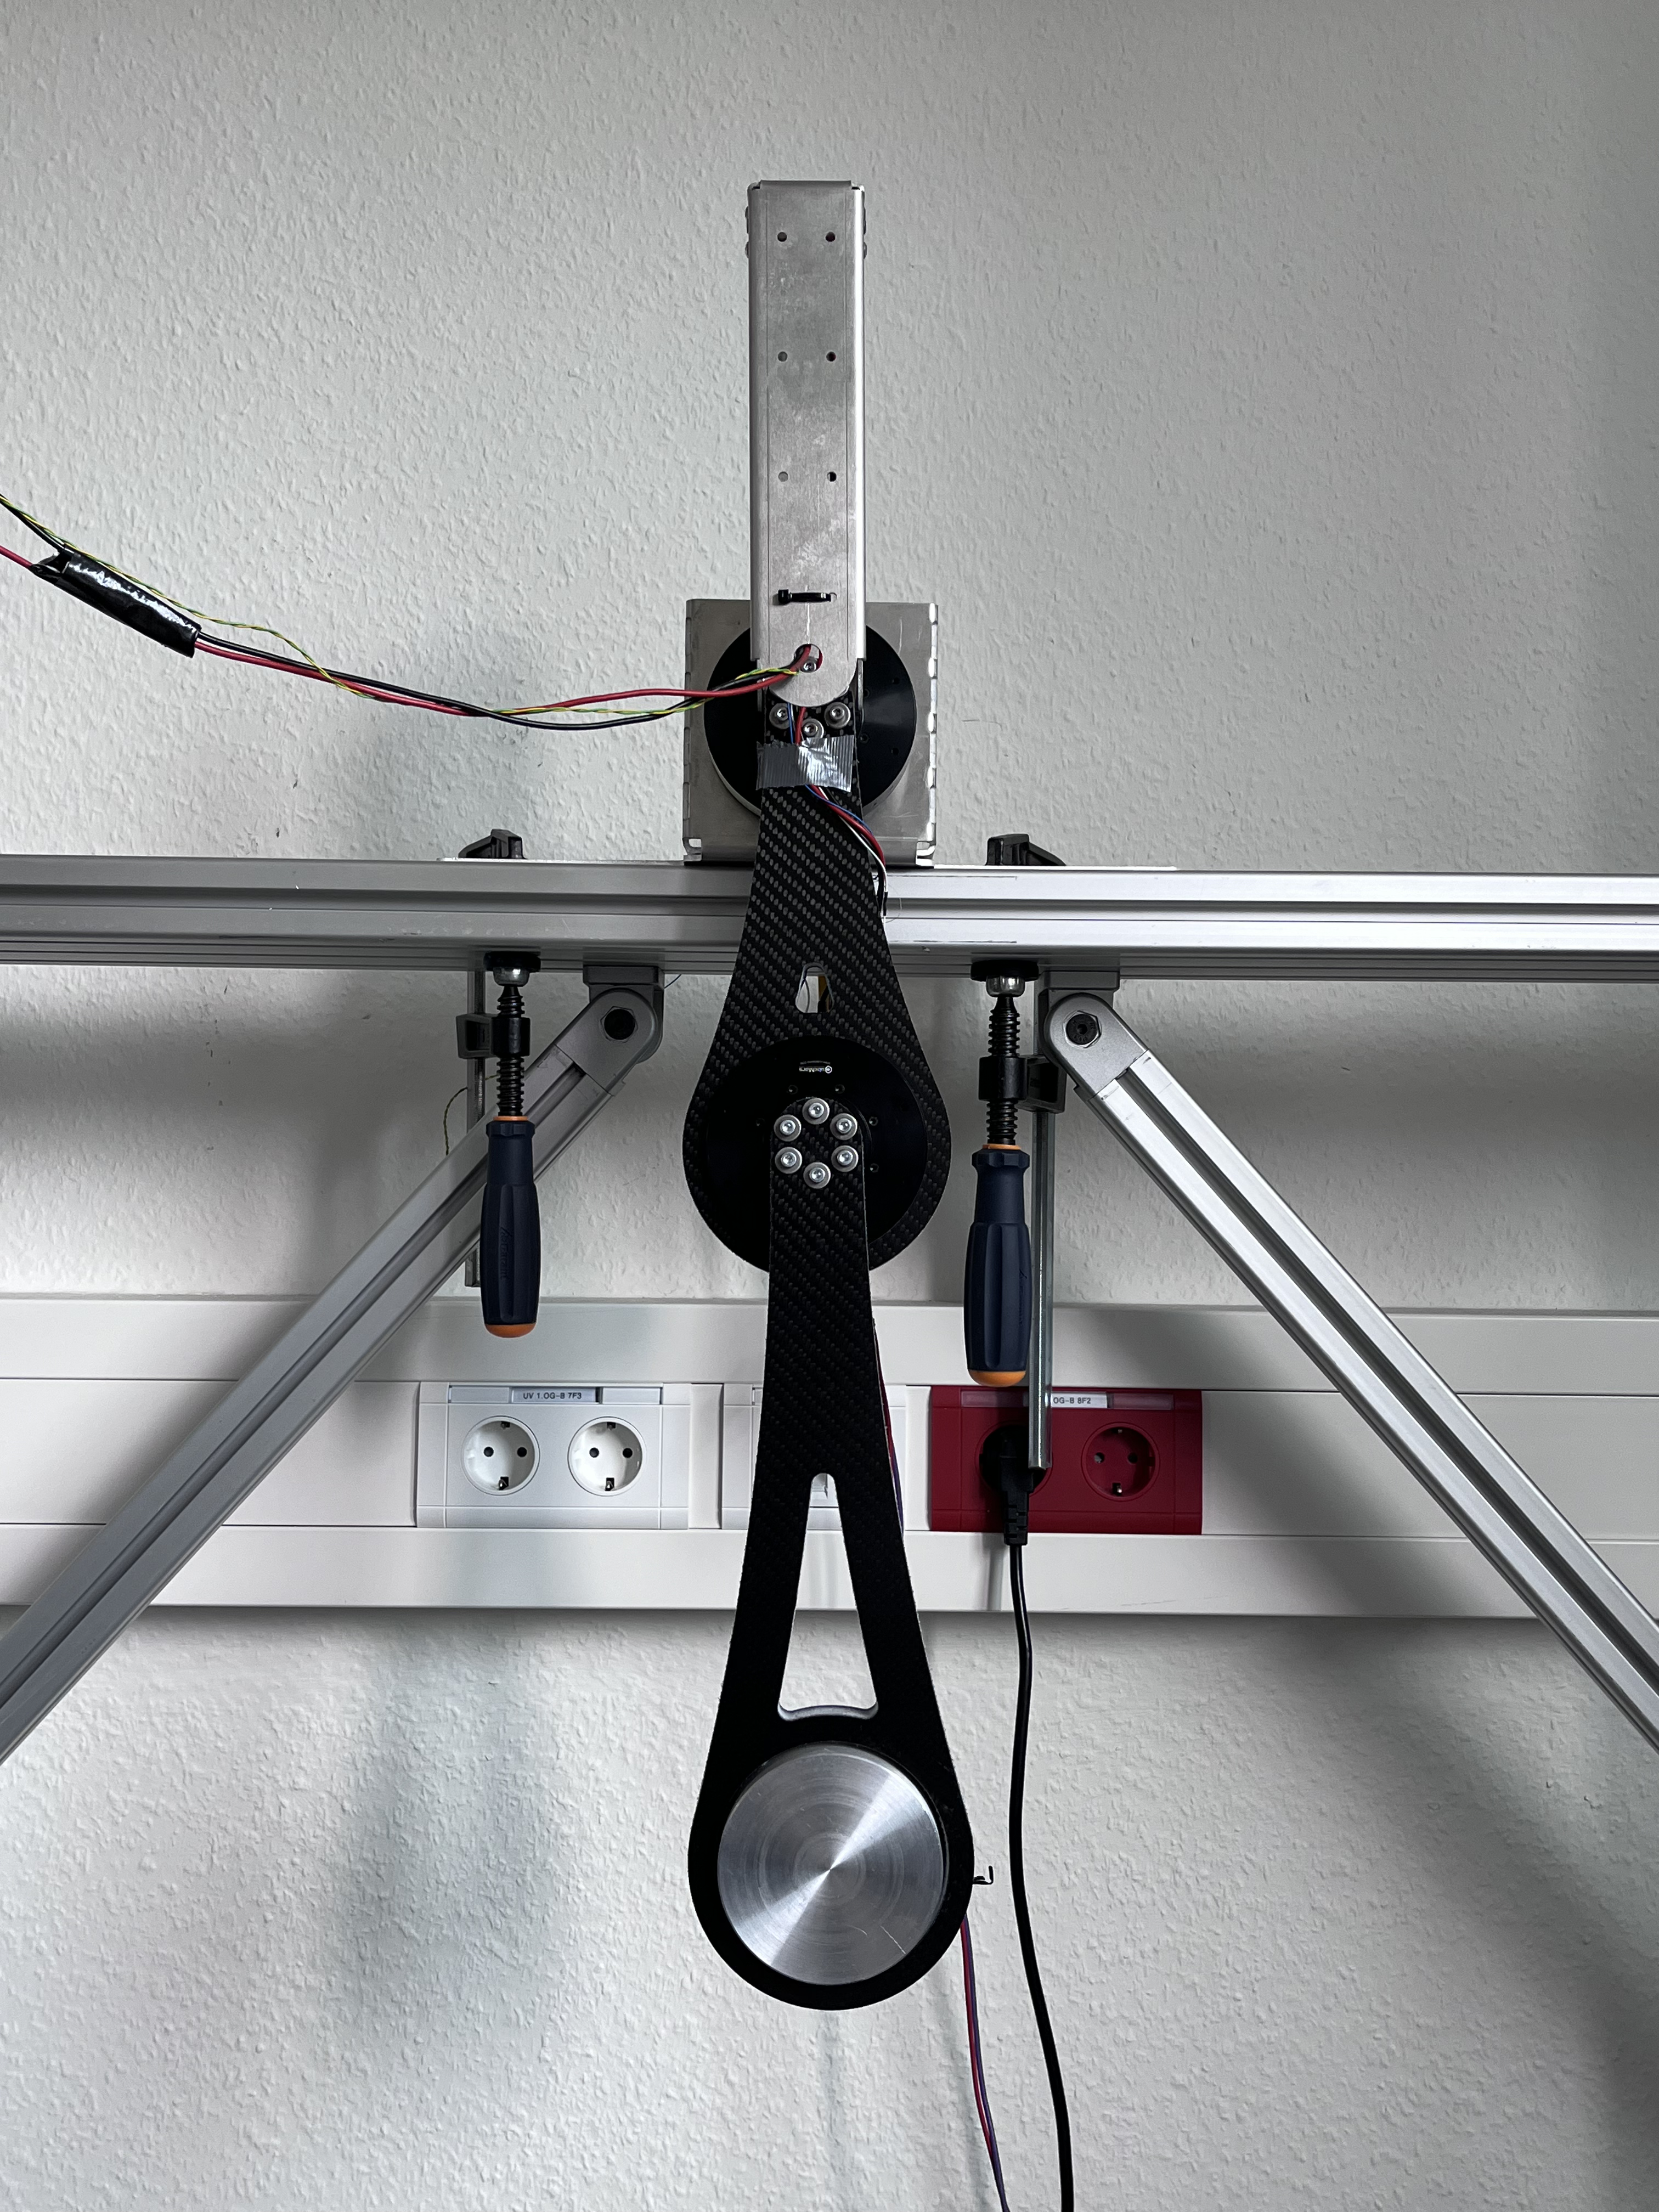
\includegraphics[width=0.45\textwidth]{figures/double_pendulum_real_system.png}
    \caption{Double pendulum in real system}
    \label{fig:image_b}
\end{figure}

The complete real-world test procedure is as follows: power up, manually set the initial state, release the emergency button, run the initialization script (which enables the motor, sets the current position to zero, and tests the CAN connection), confirm the start of the test, record video, draw plots, and exit the test. This procedure is illustrated in the flow chart below:

\begin{figure}[H]
    \centering
    \includegraphics[width=0.9\textwidth]{figures/hardware_setup/testing_procedure.png}% Second image
    \caption{Real hardware system testing procedure}
    \label{fig:image_b}
\end{figure}

Below is an example of one of our successful tests. [some explanation] We executed a sequence of 10 tests to determine the success rate and other key metrics for evaluating performance and robustness. These results will be discussed in the next chapter. 

\begin{figure}[H]
    \centering
    \includegraphics[width=1.1\linewidth]{figures/hardware_result/pendubot_real_system_working.png}
    \caption{Pendubot results on real systems}
    \label{fig:my_label}
\end{figure}


\cleardoublepage

\chapter{Discussion}
This chapter is about the discussion of results.

ad;falknv.xzfvhlsakjdgfnmdflk asdjgfmndfgb;lkjesf;mngfbl;kjfx.,mszedk.jfal;j

\section{introduction to leaderboard results}
This section is about simulation and real system leaderboard

\begin{itemize}
  \item \textbf{Swingup Success} \(c_{\text{success}}\):
  Whether the swingup was successful, i.e. if the end-effector is above the threshold line at the end of the simulation.
  
  \item \textbf{Swingup time} \(c_{\text{time}}\):
  The time it takes for the pendubot to reach the goal region above the threshold line and stay there. If the end-effector enters the goal region but falls below the line before the simulation time is over, the swingup is not considered successful! The swingup time is the time when the end-effector enters the goal region and does not leave the region until the end.
  
  \item \textbf{Energy} \(c_{\text{energy}}\):
  The mechanical energy used during the execution.
  
  \item \textbf{Max Torque} \(c_{\tau, \text{max}}\):
  The peak torque that was used during the execution.
  
  \item \textbf{Integrated Torque} \(c_{\tau, \text{integ}}\):
  The time integral over the used torque over the execution duration.
  
  \item \textbf{Torque Cost} \(c_{\tau, \text{cost}}\):
  A quadratic cost on the used torques (\(c_{\tau, \text{cost}} = \sum u^TRu\)), with \(R = 1\).
  
  \item \textbf{Torque Smoothness} \(c_{\tau, \text{smooth}}\):
  The standard deviation of the changes in the torque signal.
  
  \item \textbf{Velocity Cost} \(c_{\text{vel, cost}}\):
  A quadratic cost on the joint velocities that were reached during the execution (\(c_{\text{vel}} = \dot{q}^T Q \dot{q}\)), with \(Q = \text{identity}\).
\end{itemize}


\begin{equation}
\begin{aligned}
S = c_{\text{success}} \Bigg(& w_{\text{time}}\frac{c_{\text{time}}}{n_{\text{time}}} + \\
& w_{\text{energy}}\frac{c_{\text{energy}}}{n_{\text{energy}}} +
w_{\tau, \text{max}}\frac{c_{\tau, \text{max}}}{n_{\tau, \text{max}}} +
w_{\tau, \text{integ}}\frac{c_{\tau, \text{integ}}}{n_{\tau, \text{integ}}} + \\
& w_{\tau, \text{cost}}\frac{c_{\tau, \text{cost}}}{n_{\tau, \text{cost}}} +
w_{\tau, \text{smooth}}\frac{c_{\tau, \text{smooth}}}{n_{\tau, \text{smooth}}} +
w_{\text{vel, cost}}\frac{c_{\text{vel, cost}}}{n_{\text{vel, cost}}} \Bigg)
\end{aligned}
\end{equation}



\section{interpretation of simulation results}
This section is about explaining the simulation results.

\begin{table}
 % \begin{tabularx}{0.55\textwidth} {
 %  | >{\raggedright\arraybackslash}X
 %  | >{\centering\arraybackslash}X
 %  | >{\raggedleft\arraybackslash}X| }
  \centering
 \begin{tabular}{lcc}
 %\hline
  Criteria& Pendubot  & Acrobot \\
 \hline
 Swingup Success& success  & success\\
 %\hline
 Swingup time [s]& 0.65   & 2.06\\
 %\hline
 Energy [J]& 9.4  & 29.24 \\
 %\hline
 Max. Torque [Nm]& 5.0   & 5.0 \\
 %\hline
 Integrated Torque [Nm]& 2.21  & 4.57 \\
 %\hline
 Torque Cost [N²m²] & 8.58  & 12.32 \\
 %\hline
 Torque Smoothness [Nm]& 0.172 & 0.954 \\
 %\hline
 Velocity Cost [m²/s²]& 44.98 & 193.78  \\
 %\hline
 RealAI Score & 0.801 & 0.722  \\
 %\hline
% \end{tabularx}
 \end{tabular}
 \caption{Performance scores of our controller for pendubot and acrobot.}
 \label{tab:performance}
\end{table}

\section{interpretation of hardware results}
This section is about explaining the hardware results.

\begin{table}
 % \begin{tabularx}{0.55\textwidth} {
 %  | >{\raggedright\arraybackslash}X
 %  | >{\centering\arraybackslash}X
 %  | >{\raggedleft\arraybackslash}X| }
  \centering
 \begin{tabular}{lcc}
 %\hline
  Criteria& Pendubot  & Acrobot \\
 \hline
 Swingup Success& success  & insuccess\\
 %\hline
 Swingup time [s]& 0.67   & -\\
 %\hline
 Energy [J]& 37.12  & - \\
 %\hline
 Max. Torque [Nm]& 5.0   & - \\
 %\hline
 Integrated Torque [Nm]& 24.87  & - \\
 %\hline
 Torque Cost [N²m²] & 78.7  & - \\
 %\hline
 Torque Smoothness [Nm]& 0.774 & - \\
 %\hline
 Velocity Cost [m²/s²]& 114.04 & -  \\
 %\hline
 RealAI Score & 0.298 & -  \\
 %\hline
% \end{tabularx}
 \end{tabular}
 \caption{Real hardware performance scores of our controller for pendubot and acrobot.}
 \label{tab:performance}
\end{table}

\section{future work}
This section is to talk about things to be done.

\cleardoublepage

\chapter{Future work}
Due to the ineffectiveness of our method in real-world tests, several aspects of future work are worth exploring.

\textbf{Modify the Training Process for More Accurate Behavior Guidance:}

The unsuccessful training of an agent for the acrobot setup within speed and position limits has highlighted the necessity for an improvement in behavior guidance during training. Our current reward function only indicates to the agent to swing up and enter the Region of Attraction (RoA) of a predefined LQR controller; it doesn't provide detailed instructions on how the swing-up should be executed. Future work could base the reward function and termination conditions on mirroring a feasible trajectory within constraints.

\textbf{Model-Based Reinforcement Learning:}

As indicated in Tables \ref{tab:performance_ideal}, \ref{tab:robustness}, and \ref{tab:performance_real}, the MC-PILCO controller, as a representative of model-based reinforcement learning (MBRL) methods, delivers astonishing results. Although MBRL methods are still in their infancy, the idea of combining transition model information with pure trial-and-error shows high potential for solving complex issues like chaotic system control in real-world applications. This direction holds the most promise for achieving significant improvement in our current control problems with pendubot and acrobot setups.

\textbf{More Effective Sim-to-Real Methods}

The results presented in Table \ref{tab:performance_real} indicate a considerable need for improvements in real-world tests when SAC+LQR control is employed. The sim-to-real gap poses a challenge that limits the practical application of the SAC+LQR controller in real-world scenarios. Addressing this issue may involve several potential strategies: 

Firstly, the integration of more accurate real-world features into the learning process should be considered to enable agents to adapt to real-world complexities through trial and error, thereby enabling a smoother transition to actual systems. 

Secondly, the training of agents could be approached using direct real-world data, or by combining agent training with on-site testing on actual hardware, necessitating the use of highly sample-efficient algorithms. 

Lastly, the development of a mapping mechanism for translating results from idealized environments to the real world could be advantageous. Such a mechanism could be embodied in a neural network-based mapping function that processes state information from both simulated and real environments and actions generated for the ideal environment, outputting actions suitable for the real-world system.

\cleardoublepage

% \include{01_Chapters/03_...}
%%%%%%%%%%%%%%%%%%%%%%%%%%%%%%%%%%%%%%%%%%%%%%%%%%%%%%%%%%%%%%%%%%%%%%%%%%%%%%%%




% BIBLIOGRAPHY AND APPENDIX
%%%%%%%%%%%%%%%%%%%%%%%%%%%%%%%%%%%%%%%%%%%%%%%%%%%%%%%%%%%%%%%%%%%%%%%%%%%%%%%%
\cleardoubleemptypage
\printbibliography[heading=bibintoc] % Literature
% Appendix (optional, comment out if not needed)
% \cleardoubleemptypage
% \begin{appendices}
% 	\chapter{An appendix}

You can structure appendices, just like your thesis, with the \verb*|\chapter|, \verb*|\section|, and \verb*|\subsection| commands. Referencing also works as usual.

If your thesis does not contain an appendix, comment out the creation of the appendix at the appropriate place in the \texttt{Thesis.tex} file.
% \end{appendices}
%%%%%%%%%%%%%%%%%%%%%%%%%%%%%%%%%%%%%%%%%%%%%%%%%%%%%%%%%%%%%%%%%%%%%%%%%%%%%%%%
\end{document}
